\documentclass[12pt]{article}
\usepackage{preamble}

\pagestyle{fancy}
\fancyhead[LO,LE]{Теория вероятности}
\fancyhead[RO,RE]{Лекции Блаженова А. В.}

\fancyfoot[L]{\scriptsize исходники найдутся тут: \\ \url{https://github.com/pelmesh619/itmo_conspects} \Cat}

\renewcommand{\thesection}{}

\begin{document}

    \tableofcontents
    \clearpage

    % begin probtheory_2024_09_03.tex

    \section{Лекция 1}

    В теории вероятности обычно изучают случайные события

    Обычно наука занимается закономерностями, но так как в случайных экспериментах нет закономерностей, теория
    вероятности занимается поисков закономерности в сериях случайных экспериментах

    Итак, в XVI веке начали с экспериментов бросков монеты:

    \begin{tabular}{ccc}
        число бросков & число гербов & частота \\
        4040 & 2048 & 0.5069 \\
        12000 & 6019 & 0.5016 \\
        24000 & 12012 & 0.5005 \\
    \end{tabular}

    Как можно видеть, частота стремится к 0.5 - появляется статистическая закономерность

    \subsection{Статистическое определение вероятности}

    Пусть проводится $n$ реальных экспериментов, при которых событие $A$ появилось $n_A$ раз

    Отношение $\frac{n_A}{n}$ называется частотой события $A$

    Эксперименты показывают, что при увеличении числа $n$ частота стабилизируется у некоторого числа,
    при котором мы понимаем статистическую вероятность: $P(A) \approx \frac{n_A}{n}$ при $n \to \infty$

    \subsection{Пространство элементарных исходов. Случайные события}

    \Def Пространством элементарных исходов $\Omega$ называется множество, содержащее все возможные исходы
    экспериментов, из которых при испытании происходит ровно один. Элементы этого множества называются
    элементарными исходами и обозначаются $\omega$

    \Def Случайными событиями называется подмножество $A \subset \Omega$. События $A$ наступают, если произошел один из
    элементарных исходов из множества $A$

    \ExN{1} Бросок монеты: $\Omega = \{\text{Г}, \text{Р}\}$, $A = \{\text{Г}\}$ - выпал герб

    \ExN{2} Игральная кость: $\Omega = \{1, 2, 3, 4, 5, 6\}$, $A = \{\text{выпало четное число}\} = \{2, 4, 6\}$

    \ExN{3} Монета бросается дважды.

    a) Учитываем порядок: $\Omega = \{\text{ГГ}, \text{РР}, \text{РГ}, \text{ГР}\}$

    a) Не учитываем порядок: $\Omega = \{\text{ГГ}, \text{РР}, \text{ГР}\}$

    \ExN{4} Кубик дважды: $\Omega = \{\Pair{i, j} \ | \ 1 \leq i, j \leq 6\}$

    $A = \{\text{разность} \ \vdots \ 3\} = \{\Pair{1, 4}; \Pair{4, 1}; \Pair{2, 5}; \Pair{5, 2}; \dots\}$

    \ExN{5} Монета бросается до первого герба: $\Omega = \{\text{Г}, \text{РГ}, \text{РРГ}, \dots\}$ - счетно-бесконечное множество

    \ExN{6} Монета бросается на плоскость: $\Omega = \{\Pair{x, y} \ | \ x, y \in \Real, \Pair{x, y} \text{ - центр монеты}\}$ - несчетное число исходов

    \sebsection{Операции над событиями}

    $\Omega$ - достоверные события (наступают всегда)

    $\emptyset$ - невозможное события (никогда не наступает, так как не содержит ни одного элем. исхода)

    Введем операции:

    \DefN{1} Суммой $A + B$ называется событие, состоящее в том, что произошло события $A$ или событие $B$ (хотя бы одно из них)

    \DefN{2} Произведением $A \cdot B$ называется событие, состоящее в том, что произошло событие $A$ и событие $B$ (оба из них)

    \Notas $A_1 + A_2 + \dots + A_n + \dots$ - произошло хотя бы одно из этих событий

    $A_1 \cdot A_2 \cdot \dots \cdot A_n \cdot \dots$ - произошли все эти события

    \DefN{3} Противоположным $A$ событием называется событие $\overline{A}$, состоящее в том, что событие $A$ не произошло

    \Notas $\overline{A} = A$ % не понял почему

    \DefN{4} Дополнение (разность) $A \setminus B$ называется событие $A \cdot \overline{B}$

    \DefN{5} События $A$ и $B$ называются несовместными, если их произведение - пустое множество
    (не могут произойти одновременно при одной эксперименте)

    \DefN{6} События $A$ влечет события $B$, если $A \subset B$ (если наступает $A$, то наступит $B$)

    \subsection{Вероятность}

    Мы хотим присвоить какую-то числовую характеристику к каждому событию,
    отражающее его частоту наступления: $0 \leq P(A) \leq 1$ - вероятность наступления события $A$

    \mediumvspace

    \textbf{Классическое определение вероятности}

    Пусть пространство случайных событий $\Omega$ содержит конечное число равновозможных исходов,
    тогда применимо классическое определение вероятности

    \Def \fbox{$P(A) = \frac{|A|}{|\Omega|} = \frac{m}{n}$}, где $n$ - число всех возможных исходов, $m$ - число благоприятных исходов

    В частности, если $\Omega = n$ и $A_i$ - элем. исх., то $P(A_i) = \frac{1}{n}$

    Свойства:

    1) $0 \leq P(A) \leq 1$

    2) $P(\Omega) = 1 \quad (m = n)$

    3) $P(\emptyset) = 0 \quad (m = 0)$

    4) Если события $A$ и $B$ несовместны, то $P(A + B) = P(A) + P(B)$

    \mediumvspace

    \textbf{Геометрическое определение вероятности (граф де Бюффон)}

    Пусть $\Omega \subset \Real^n$ - замкнутая ограниченная область

    $\mu(\Omega)$ - мера $\Omega$ в $\Real^n$ (например, длина отрезка, площадь области на плоскости, объем тела в пространстве)

    В эту область наугад бросаем точку. \enquote{Наугад} означает, что вероятность попадания в $A$ зависит только от меры $A$ и не зависит от ее расположения

    В этом случае применимо геометрическое определение вероятности

    $P(A) = \frac{\mu(A)}{\mu(\Omega)}$

    \ExN{1} Монета диаметром в 6 см бросается на пол, вымощенной квадратной плиткой со стороной 20 см, какова вероятность,
    что монета окажется целиком внутри одной плитки

    $\mu(\Omega) = 20^2 = 400$

    $\mu(A) = (20 - 3 - 3)^2 = 196$

    $P(A) = \frac{\mu(A)}{\mu(\Omega)} = \frac{196}{400} = 0.49$

    \hypertarget{buffonsproblem}{}

    \ExN{2} Задача Бюффона об игле: пусть пол вымощен ламинатом, $2l$ - ширина доски, на пол бросается игла длины, равной ширине доски,
    найти вероятность того, что игла пересечет стык доски

    \smallvspace

    \begin{minipage}{\linewidth}
        \begin{wrapfigure}{r}{0pt}
            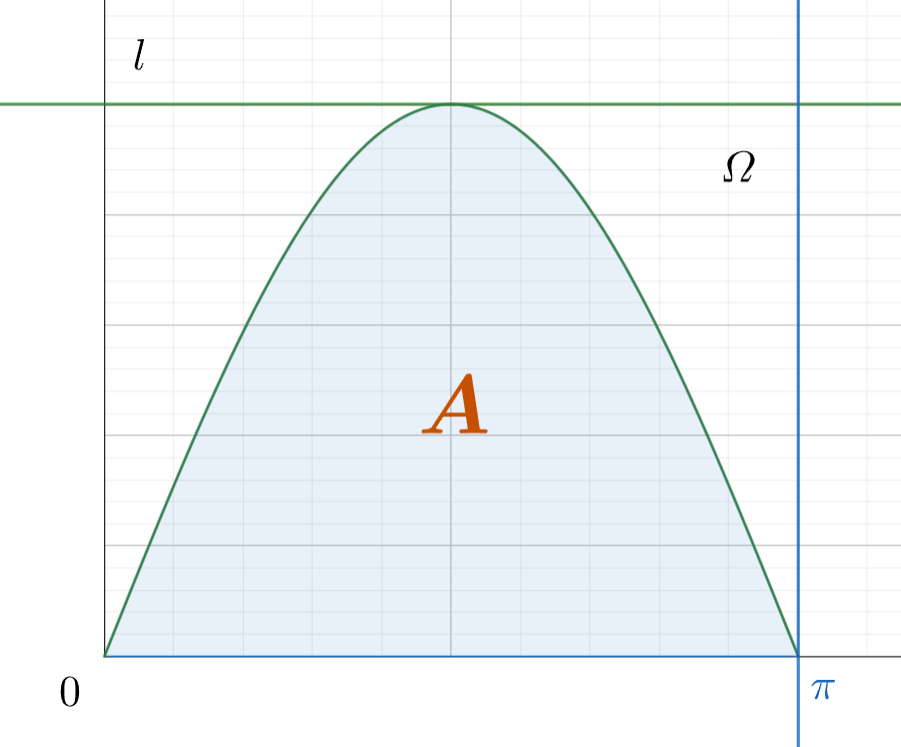
\includegraphics[height=6cm]{probtheory/images/probtheory_2024_09_03_1}
        \end{wrapfigure}

        Определим положение иглы координатами центра и углом, между иглой и стыком доски, причем можно считать, что эти величины независимы

        $\letsymbol x \in [0; l]$ - расстояние от центра до ближайшего края, $\varphi \in [0; \pi]$ - угол

        $\Omega = [0; l] \times [0; \pi]$

        Событие $A$ (пересечет стык) наступает, если $x \leq l \sin \varphi$

        $P(A) = \frac{S(A)}{S(\Omega)}$

        $S(\Omega) = \pi l$

        $S(A) = \int_0^\pi l \sin \varphi d\varphi = -l \cos \varphi \Big|_0^\pi = -l (-1 - 1) = 2l$

        $P(A) = \frac{2l}{\pi l} = \frac{2}{\pi}$
    \end{minipage}
% end probtheory_2024_09_03.tex

% begin probtheory_2024_09_10.tex

    \section{Лекция 2}
    
    \subsection{Построение модели случайных явлений}

    \begin{enumerate}
        \item Задаем пространство элементарных исходов $\Omega$

        \item \Defs Система $\mathcal{F}$ подмножеств $\Omega$ называется $\sigma$-алгеброй событий, если:

        1) $\Omega \in \mathcal{F}$;

        2) $A \in \mathcal{F} \Longrightarrow \overline{A} \in \mathcal{F}$;

        3) $A_1, A_2, \dots, A_n, \dots \in \mathcal{F} \Longrightarrow \bigunion_{i = 1}^\infty A_i \in \mathcal{F}$

        \textbf{Свойства}:

        \begin{enumerate}
            \item $\emptyset \in \mathcal{F}$, так как $\Omega \in \mathcal{F} \Longrightarrow \overline{\Omega} = \emptyset \in \mathcal{F}$

            \item $A_1, A_2, \dots \in \mathcal{F} \Longrightarrow \bigcap_{i = 1}^\infty A_i \in \mathcal{F}$

            \begin{tcolorbox}
                $\Box \quad$ $A_1, A_2, \dots \in \mathcal{F} \Longrightarrow
                \overline{A}_1, \overline{A}_2, \dots \in \mathcal{F} \Longrightarrow
                \bigunion_{i = 1}^\infty \overline{A}_i \in \mathcal{F} \Longrightarrow
                \overline{\bigunion_{i = 1}^\infty \overline{A_i}} = \bigcap_{i = 1}^\infty A_i \in \mathcal{F} \quad \Box$
            \end{tcolorbox}

            \item $A, B \in \mathcal{F} \Longrightarrow A \setminus B \in \mathcal{F}$

            \begin{tcolorbox}
                $\Box \quad$ $A, B \in \mathcal{F} \Longrightarrow A, \overline{B} \in \mathcal{F} \Longrightarrow A \setminus B = A \cdot \overline{B} \in \mathcal{F}$ $\quad \Box$
            \end{tcolorbox}

        \end{enumerate}

        \ExNs{1} $\mathcal{F} = \{\emptyset, \Omega\}$

        \ExNs{2} $\mathcal{F} = \{\emptyset, \Omega, A, \overline{A}\}$

        \ExNs{3} \Defs Борелевская $\sigma$-алгебра $\mathcal{B}(\Real)$ - минимальная $\sigma$-алгебра, содержащая все возможные интервалы на прямой

        % на плоскости борелевская сигма-алгебра - прямоугольники

        \item \Defs $\letsymbol\ \Omega$ - пространство элементарных исходов, $\mathcal{F}$ - его $\sigma$-алгебра событий.
        \textit{Вероятностью} на $(\Omega, \mathcal{F})$ называется функция $P: \mathcal{F} \to \Real$ со свойствами:

        \begin{enumerate}
            \item $P(A) \geq 0 \quad \forall A \in \mathcal{F}$ (неотрицательность)

            \item Если $A_1, A_2, \dots, A_n, \dots \in \mathcal{F}$ - несовместное, то $P(\sum_{i = 1}^\infty A_i) = \sum_{i = 1}^\infty P(A_i)$ (свойство счетной аддитивности)

            \item $P(\Omega) = 1$ (условие нормированности)
        \end{enumerate}

    \end{enumerate}

    \Def Из этого тройка $(\Omega, \mathcal{F}, P)$ называется вероятностным пространством

    \subsection{Свойства вероятности}

    \begin{enumerate}

        \item Так как $\emptyset$ и $\Omega$ - несовместные, то $1 = P(\Omega) = P(\Omega + \emptyset) = 1 + P(\emptyset) \Longrightarrow P(\emptyset) = 0$

        \item Формула обратной вероятности: $P(A) = 1 - P(\overline{A})$

        \begin{tcolorbox}
            $\Box \quad$ $A$ и $\overline{A}$ - несовместные и $A + \overline{A} = \Omega \Longrightarrow P(A + \overline{A}) = P(\Omega) = 1$ $\quad \Box$
        \end{tcolorbox}

        \item $P(A) = 1 - P(\overline{A}) \leq 1$

    \end{enumerate}

    \subsection{Аксиома непрерывности}

    Пусть имеется убывающая цепочка событий $A_1 \supset A_2 \supset A_3 \supset \dots \supset A_n \supset \dots$ и $\bigcap_{i = 1}^\infty A_n = \emptyset$

    Тогда $P(A_n) \underset{n \to \infty}{\to} 0$

    При непрерывном изменении области $A \subset \Omega \subset \Real^n$ соответствующая вероятность $P(A)$ также должна изменятся непрерывно

    \Th Аксиома непрерывности следует из аксиомы счетной аддитивности

    \begin{tcolorbox}
        $\Box$

        Ясно, что $A_n = \sum_{i = n}^\infty A_i \overline{A}_{i + 1} + \prod_{i = n}^\infty A_i$

        $\prod_{i = n}^\infty A_i = A_n \cdot \prod_{i = n + 1}^\infty A_i = \prod_{i = 1}^n
        \cdot \prod_{i = n + 1}^\infty A_i = \prod_{i = 1}^\infty = \emptyset \Longrightarrow
        A_n = \sum_{i = n}^\infty A_n \overline{A_{n + 1}}$ и так как эти события несовместны,
        то по свойству счетной аддитивности $P(A_n) = \sum_{i = n}^\infty P(A_i \overline{A_{i + 1}})$ - это остаток (хвост) сходящегося ряда

        $P(A_1) = \sum_{i = 1}^\infty P(A_i \overline{A_{i + 1}}) = \sum_{i = 1}^{n - 1} P(A_i \overline{A_{i + 1}}) + P(A_n)$ и $P(A_n) \underset{n \to \infty}{\to} 0$ по необходимому признаку сходимости

        $\Box$
    \end{tcolorbox}

    \Nota Аксиому счетной аддитивности можно вывести из конечной аддитивности и аксиомы счетной непрерывности

    \textbf{Свойства операций сложения и умножения}

    1. Свойство дистрибутивности: $A \cdot (B + C) = AB + AC$

    2. Формула сложения: если $A$ и $B$ несовместны, то $P(A + B) = P(A) + P(B)$

    3. Формула сложения вероятностей: $P(A + B) = P(A) + P(B) - P(AB)$

    \begin{tcolorbox}
        $\Box$

        $A + B = A\overline{B} + AB + \overline{A}B$ - несовместные события $\Longrightarrow P(A + B) = P(A\overline{B}) + P(AB) + P(\overline{A}B) =
        (P(A\overline{B}) + P(\overline{A}B)) - P(AB) = P(A) + P(B) - P(AB)$

        $\Box$
    \end{tcolorbox}

    \Ex Из колоды в 36 карт достали одну карту. Какова вероятность того, что будет дама или пика

    Пусть Д - дама, П - пика, $P(\text{Д} + \text{П}) = P(\text{Д}) + P(\text{П}) - P(\text{Д}\text{П}) = \frac{4}{36} + \frac{9}{36} - \frac{1}{36} = \frac{1}{3}$

    Формула сложения при $N = 3$: $P(A_1 + A_2 + A_3) = P(A_1) + P(A_2) + P(A_3) - P(A_2 A_3) - P(A_1 A_3) - P(A_1 A_2) + P(A_1 A_2 A_3)$

    Общий случай: $P(A_1 + A_2 + \dots + A_n) =  \sum_{i = 1}^n P(A_i) - \sum_{i < j} P(A_i A_j) + \sum_{i < j < k} P(A_i A_j A_k) + (-1)^{n - 1} \cdot P(A_1 A_2 \dots A_n)$ - формула включения и исключения

    \Ex $n$ писем случайно раскладывается по $n$ конвертам. Найти вероятность того, что хотя бы одно письмо окажется в своем конверте

    $\letsymbol A_i$ - $i$-ое письмо в своем конверте

    $P(A_i) = \frac{1}{n}; P(A_i A_j) = \frac{1}{A^2_n}; P(A_i A_j A_k) = \frac{1}{A^3_n}; P(A_1 A_2 \dots A_n) = \frac{1}{n!}$

    Слагаемых вида $A_i$ - $n$ штук; $A_i A_j$ - $C^2_n$; $A_i A_j A_k$ - $C^3_n$; $A_1 A_2 \dots A_n$ - 1 штука

    $P(A) = P(A_1 + A_2 + \dots + A_n) = n \cdot \frac{1}{n} - C^2_n \frac{1}{A^2_n} + C^3_n \frac{1}{A^3_n} - \dots + (-1)^{n - 1} \frac{1}{n!} = 1 - \frac{1}{2} + \frac{1}{3!} - \dots + (-1)^{n - 1} \frac{1}{n!}$

    Так как $e^{-1} = 1 - 1 + \frac{1}{2} - \frac{1}{3!} + \dots$, то при $n \to \infty \quad P(A) \underset{n \to \infty}{\to} 1 - e^{-1} \approx 0.63$

    Независимые события

    Под независимыми событиями логично подразумевать события, не связанные причинно-следственной связью (то есть когда факт наступления одного не влияет на оценку вероятности другого)

    $\letsymbol |\Omega| = n; |A| = m_1; |B| = m_2$

    Проведем пару независимых испытаний. Тогда получаем пространство элементарных исходов $\Omega \times \Omega$ и $|\Omega \times \Omega| = n^2$

    По основному принципу комбинаторики $|A \cdot B| = m_1 \cdot m_2$

    $P(AB) = \frac{|A \cdot B|}{|\Omega \times \Omega|} = \frac{m_1 m_2}{n^2} = P(A) \cdot P(B)$

    \Def События $A$ и $B$ называются независимыми, если $P(A \cdot B) = P(A) \cdot P(B)$

    \Lab $\letsymbol P(A), P(B) \neq 0$, доказать, что если $A$ и $B$ несовместны, то они зависимы

    Свойство: Если $A$ и $B$ независимы, то независимы $\overline{A}$ и $\overline{B}$, $A$ и $\overline{B}$, $\overline{A}$ и $B$

    Доказательство: $A = A \cdot (B + \overline{B}) = AB + A\overline{B}$ - несовместные события $\Longrightarrow P(A) = P(AB) + P(A\overline{B}) \Longrightarrow P(A\overline{B}) = P(A) - P(AB) =
    P(A) - P(A) \cdot P(B) = P(A) (1 - P(B)) = P(A) P(\overline{B}) \Longrightarrow$ независимы

    \Def События $A_1, A_2, \dots A_n$ - независимы в совокупности, если для любого набора $i_1, i_2, \dots, i_k \ (2 \leq k \leq n)$
    $P(A_{i_1} \cdot A_{i_2} \cdot \dots \cdot A_{i_k}) = P(A_{i_1}) \cdot P(A_{i_2}) \cdot \dots \cdot P(A_{i_k})$

    \Nota Из независимости в совокупности при $k = 2$ получаем попарную независимость. Обратное утверждение неверно

    \Ex (С. Бернштейн)

    Пусть имеется правильный тетраэдр, одна грань окрашена в красный, вторая в синий, третья в зеленый, а четвертая во все эти три цвета.

    Подбросили тетраэдр, $\letsymbol A$ - грань, которая содержит красный цвет, $B$ - синий, $C$ - зеленый.

    $P(A) = P(B) = P(C) = \frac{2}{4} = \frac{1}{2}$

    Так как $P(AB) = P(AC) = P(BC) = \frac{1}{4}$

    $P(AB) = \frac{1}{4} = \frac{1}{2} \cdot \frac{1}{2} = P(A) P(B)$ - попарная независимость

    $P(ABC) = \frac{1}{4} \neq P(A) P(B) P(C)$ - но вот независимость в совокупности не соблюдается

    \Ex (Шевалье де Мере, Паскаль, Ферма, $\approx$ 1650 г.)

    Какова вероятность того, что при 4 бросании кости выпадет одна шестерка

    $A_1$ - при первом броске шестерка, $A_2$ - при втором, $A_3$ - при третьем, $A_4$ - при четвертом

    $B$ - выпала хотя бы одна шестерка при 4 бросках

    $B = A_1 + A_2 + A_3 + A_4$ - совместные события, но независимые

    Найдем обратную вероятность: $\overline{B}$ - ни разу не выпала шестерка

    $\overline{B} = \overline{A_1} \cdot \overline{A_2} \cdot \overline{A_3} \cdot \overline{A_4}$

    $P(\overline{A_1}) = P(\overline{A_2}) = P(\overline{A_3}) = P(\overline{A_4}) = \frac{5}{6}$

    $\overline{B} = P(\overline{A_1}) P(\overline{A_2}) P(\overline{A_3}) P(\overline{A_4}) = \left(\frac{5}{6}\right)^4 \approx 0.482$

    $P(B) = 1 - P(\overline{B}) \approx 0.52$
% end probtheory_2024_09_10.tex

% begin probtheory_2024_09_17.tex

    \section{Лекция 3}

    \subsection{Условная вероятность}

    Условная вероятность $P(A|B)$ (или $P_B(A)$) - вероятность события $A$, вычисленная в предположении, что событие $B$ уже произошло

    \Ex Бросается кость один раз, известно, что выпало больше 3 очков. Найти вероятность того, что выпало четное число очков

    \smallvspace

    \begin{minipage}{\linewidth}
        \begin{wrapfigure}{r}{0pt}
            \begin{center}
                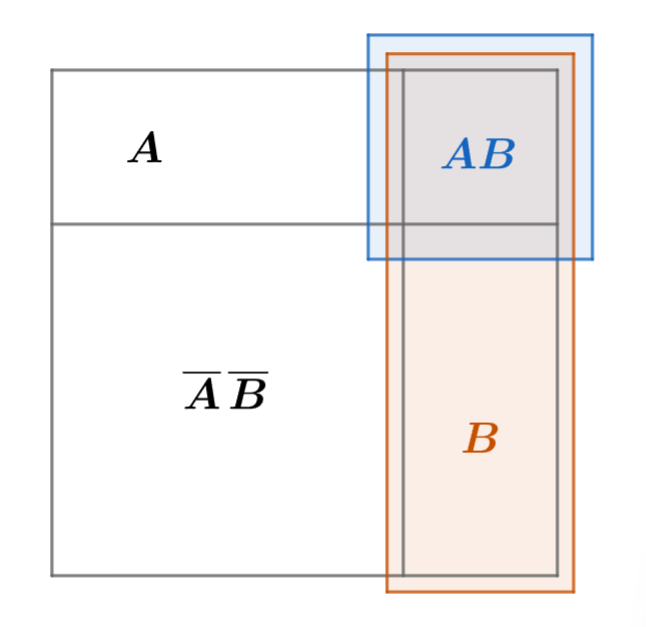
\includegraphics[height=5cm]{probtheory/images/probtheory_2024_09_17_1}
            \end{center}
        \end{wrapfigure}

        $A$ - выпало четное число очков

        $B$ - выпало больше трех очков

        $\Omega = \{1, 2, 3, 4, 5, 6\}; |\Omega| = 6; A = \{2, 4, 6\}; B = \{4, 5, 6\}$

        $P(A|B) = \frac{2}{3} = \frac{\frac{2}{6}}{\frac{3}{6}} = \frac{P(AB)}{P(B)}$


        Интерпретация с помощью геометрической вероятности:

        $P(A|B) = \frac{S_{AB}}{S_B} = \frac{\frac{S_{AB}}{S_\Omega}}{\frac{S_B}{S_\Omega}}$
    \end{minipage}

    \Def Условной вероятностью события $A$ при условии, что имело место событие $B$, называется величина $P(A|B) = \frac{P(AB)}{P(B)}$

    \Ex Известно, что среди населения 1\% воров. В комнате, где находилось 10 гостей, у хозяина пропал кошелек. Какова вероятность того, что произвольный гость является вором.

    $A$ - гость является вором $P(A) = 0.01$

    $B$ - пропал кошелек (хотя бы один вор среди гостей есть)

    $P(A|B) = \frac{P(AB)}{P(B)} = \frac{P(AB)}{1 - P(\overline{B})} = \frac{P(A)}{1 - 0.99^{10}} = \frac{0.01}{1 - 0.99^{10}} = 0.105$

    Формула умножения:

    В качестве следствия условной вероятности получаем:

    $P(A|B) = \frac{P(AB)}{P(B)} \Longrightarrow P(AB) = P(B) \cdot P(A|B) = P(A) \cdot P(B|A)$

    Общий случай:

    $P(A_1 A_2 A_3 \dots A_n) = P(A_1) P(A_2 | A_1) P(P_3 | A_1 A_2) \dots P(A_n | A_1 A_2 \dots A_{n - 1})$

    \begin{tcolorbox}
        $\Box$

        База индукции $P(AB) = P(B) P(A|B)$

        Шаг индукции: пусть верно при $n - 1$:

        $P(A_1 A_2 A_3 \dots A_{n - 1}) = P(A_1) P(A_2 | A_1) P(P_3 | A_1 A_2) \dots P(A_n | A_1 A_2 \dots A_{n - 2})$

        $P(A_1 A_2 A_3 \dots A_n) = P(A_1 A_2 A_3 \dots A_{n - 1}) \cdot P(A_n | A_1 A_2 \dots A_{n - 1}) = \\
        P(A_1) P(A_2 | A_1) P(P_3 | A_1 A_2) \dots P(A_n | A_1 A_2 \dots A_{n - 1})$

        $\Box$
    \end{tcolorbox}


    \Ex Студент выучил 1 билет из $n$, в группе $n$ студентов. Каким по очереди ему нужно зайти, чтобы вероятность сдать экзамен была наибольшей

    Пусть $A_i$ - билет, вытянутый на $i$-ом шаге ($1 \leq i \leq n$)

    $A$ - студент сдал экзамен

    $P(A) = P(\overline{A_1} \cdot \overline{A_2} \cdot \dots \cdot \overline{A_{i - 1}} \cdot A_i) = \frac{n - 1}{n} \cdot \frac{n - 2}{n - 1} \cdot \dots \cdot \frac{n - (i - 1)}{n - (i - 2)} \cdot \frac{1}{n - (i - 1)} = \frac{1}{n}$

    \subsection{Полная группа событий}

    \Def События $H_1, H_2, \dots, H_n, \dots$ образуют полную группу событий, если они попарно несовместны и содержат все возможные элементарные исходы

    $H_i \cap H_j = \emptyset \ \forall i, j \quad\quad\quad \bigunion_{i = 1}^{\infty} H_i = \Omega$

    Следствие: $\sum_{i = 1}^\infty P(H_i) = 1$

    \ThN{Формула полной вероятности} $\letsymbol H_1, H_2, \dots, H_n, \dots$ - полная группа событий. Тогда $P(A) = \sum_{i = 1}^\infty P(H_i) P(A | H_i)$

    \begin{tcolorbox}
        $\Box$

        $P(A) = P(\Omega A) = P((H_1 + H_2 + H_3 + \dots) A) = P(H_1 A + H_2 A + H_3 A + \dots) = [H_i \cdot A \cdot H_j \cdot A = \emptyset \cdot A] = P(H_1 A) + P(H_2 A) + \dots =
        P(H_1) P(A | H_1) + P(H_2) P(A | H_2) + \dots$

        $\Box$
    \end{tcolorbox}

    \ThN{Формула Байеса} $\letsymbol H_1, H_2, \dots, H_n$ - полная группа событий, и известно, что событие $A$ уже произошло

    Тогда $P(H_k | A) = \frac{P(H_k) P(A | H_k)}{\sum_{i = 1}^\infty P(H_i) P(A | H_i)}$

    \begin{tcolorbox}
        $\Box$

        $P(H_k | A) = \frac{P(H_k A)}{P(A)} = \frac{P(H_k) P(A|H_k)}{\sum_{i = 1}^\infty P(H_i) P(A|H_i)}$

        $\Box$
    \end{tcolorbox}

    \ExN{1} В первой коробке 4 белых и 2 черных шара, во второй 1 белый и 2 черных. Из первой коробки во вторую переложили 2 шара, затем из второй коробки достали шар. Какова
    вероятность того, что он оказался белым

    $\letsymbol H_1$ - переложили 2 белых
    $H_2$ - 2 черных

    $H_3$ - разного цвета

    $A$ - из второй коробки достали белый шар

    $P(H_1) = \frac{4}{6} \cdot \frac{3}{5} = \frac{6}{15}$

    $P(H_2) = \frac{2}{6} \cdot \frac{1}{5} = \frac{1}{15}$

    $P(H_3) = \frac{4}{6} \cdot \frac{2}{5} + \frac{2}{6} \cdot \frac{4}{5} = \frac{4}{15} + \frac{4}{15} = \frac{8}{15}$

    $P(A) = P(H_1) \cdot P(A|H_1) + P(H_2) \cdot P(A|H_2) + P(H_3) \cdot P(A|H_3) = \frac{6}{15} \cdot \frac{3}{5} + \frac{1}{15} \cdot \frac{1}{5} + \frac{8}{15} \cdot \frac{2}{5} =
    \frac{18}{75} + \frac{1}{75} + \frac{16}{75} = \frac{35}{75} = \frac{7}{15}$

    \ExN{2} Вероятность попадания первого стрелка в цель $0.9$, а второго $0.3$. Наугад вызванный стрелок попал в цель. Какова вероятность того, что это бы первый стрелок?

    $H_1$ - вызван первый стрелок

    $H_2$ - вызван второй стрелок

    $A$ - стрелок попал

    $P(H_1) = P(H_2) = \frac{1}{2}$

    $P(A|H_1) = 0.9 \quad\quad P(A|H_2) = 0.3$

    $P(H_1 | A) = \frac{P(H_1) P(A|H_1)}{P(H_1) P(A|H_1) + P(H_2) | P(A | H_2)} = \frac{\frac{1}{2} 0.9}{\frac{1}{2} 0.9 + \frac{1}{2} 0.3} = \frac{9}{9 + 3} = 0.75$

    \ExN{3} По статистике раком болеет 1\% населения. Тест дает правильный результат в 99\% случаев. Тест оказался положительный. Найти вероятность того, что человек болен.

    $H_1$ - человек болен

    $H_2$ - человек здоров

    $A$ - анализ положительный

    $P(H_1) = 0.01$

    $P(H_2) = 0.99$

    $P(A|H_1) = 0.99$

    $P(A|H_2) = 0.01$

    $P(H_1 | A) = \frac{P(H_1)P(A | H_1)}{P(H_1) P(A | H_1) + P(H_2) P(A | H_2)} = \frac{0.01 \cdot 0.99}{0.01 \cdot 0.99 + 0.99 \cdot 0.01} = \frac{1}{2} = 0.5$

    Допустим, что второй независимый с первым анализ также оказался положительным. Найти вероятность того, что человек болен.

    $P(H_1) = 0.01 \quad\quad P(H_2) = 0.99$

    $P(AA|H_1) = 0.99^2 \quad\quad P(AA|H_2) = 0.01^2$

    $P(H_1 | AA) = \frac{0.01 \cdot 0.99^2}{0.01 \cdot 0.99^2 + 0.99 \cdot 0.01^2} = \frac{0.99}{0.99 + 0.01} = 0.99$

    Интуитивно вероятность $\frac{1}{2}$ может поддаваться непониманию, однако можно рассуждать так:
    пусть в городе живут 10000 человек, из них 100 болеют, а у 99 из них положительный анализ; у других 9900 положительный анализ всего лишь у 99, отсюда выходит $\frac{1}{2}$

    \ExN{4} В телевизионной студии 3 двери {\Large 🚪🚪🚪}, за одной из них приз {\Large 🚗}.
    Игрок выбрал наугад одну из 3 дверей, после чего ведущий открывает одну из двух оставшихся дверей и показывает, что там приза нет {\Large 🛴}. После чего
    предлагает игроку поменять свой выбор. Стоит ли игроку соглашаться?

    $H_1$ - игрок угадал

    $H_2$ - игрок не угадал

    $A$ - ведущий открыл дверь без приза

    $P(H_1) = \frac{1}{3} \quad\quad P(H_2) = \frac{2}{3}$

    $P(A|H_1) = 1 \quad\quad P(A|H_2) = \frac{1}{2}$

    $P(H_1|A) = \frac{\frac{1}{3} \cdot 1}{\frac{1}{3} \cdot 1 + \frac{1}{3} \cdot \frac{1}{2}} = \frac{1}{2}$

    Но это неправильно, так как действия ведущего неслучайны - он всегда откроет дверь без приза

    В этом случае, если мы гипотетически выберем 300 дверей, в 100 случаях мы отгадаем, ведущий откроет любую дверь без приза;
    но в 200 случаях мы не отгадаем, ведущий откроет вторую дверь без приза, и в этом случае мы сможем поменяться на дверь с призом,
    отсюда шанс $\frac{2}{3}$, если мы поменяем свой выбор \hfill


    \ExN{5} Вероятность того, что в семье с детьми ровно $k$ детей, равна $\frac{1}{2^k}$, $k = 1, 2, \dots$
    Какова вероятность того, что в семье один мальчик, если известно, что нет
    девочки? Рождения мальчиков и девочек равновероятны.


    $H_i$ - в семье $i$ детей ($1 \leq i < \infty$)

    $P(H_i) = \frac{1}{2^i}$

    $A$ - в семье нет девочки

    $P(A|H_1) = \frac{1}{2}$

    $P(A|H_2) = \frac{1}{4}$

    $P(A|H_i) = \frac{1}{2^i}$

    $P(H_1 | A) = \frac{\frac{1}{2} \frac{1}{2}}{\sum_{i = 1}^\infty \frac{1}{2^i} \cdot \frac{1}{2^i}} = \frac{\frac{1}{4}}{\frac{\frac{1}{4}}{1 - \frac{1}{4}}} = \frac{3}{4} = 0.75$
% end probtheory_2024_09_17.tex

% begin probtheory_2024_09_24.tex

    \section{Лекция 4}

    \subsection{Серия испытаний Бернулли}

    Схемой Бернулли - называется серия одинаковых независимых экспериментов, каждый из которых имеет 2 исхода: произошло интересующее нас событие или нет

    $p = p(A)$ - вероятность успеха при одном испытании

    $q = 1 - p$ - вероятность неудачи

    $v_n$ - число успехов в серии из $n$ испытаний

    $p(v_n = k) = p_n(k)$

    Из этого получаем формулу Бернулли:

    \begin{MyTheorem}
        \Ths Вероятность того, что при $n$ испытаниях произойдет ровно $k$ успехов, равна

        $p_n(k) = C_n^k p^k q^{n - k}$
    \end{MyTheorem}

    \begin{MyProof}
        $\Box$

        Рассмотрим один из элементарных исходов, благоприятных данному событию:

        $A_n = \underset{k}{\underbrace{\text{УУУ}\dots\text{У}}}\underset{n - k}{\underbrace{\text{Н}\dots\text{ННН}}}$ - $k$ успехов, $n - k$ неудачи

        $p(\text{У}) = p, p(\text{Н}) = q$

        Так как испытания независимы, то $p(A_n) = p^k q^{n - k}$

        Остальные элементарные исходы имеют ту же вероятность, перебираем все расстановки исходов, получаем $C_n^k$, в итоге, получаем формулу Бернулли

        $\Box$
    \end{MyProof}

    \Ex Вероятность попадания стрелка при одном выстреле - $0.8$. Какова вероятность того, что из пяти выстрелов точными будут три

    $n = 5 \quad p = 0.8 \quad q = 1 - p = 0.2 \quad k = 3$

    $p_5(3) = C^3_5 p^3 q^2 = 0.2048$

    \subsection{Наиболее вероятное число успехов}

    Выясним, при каком значении $k$ вероятность предшествующего числа успехов $k - 1$ будет не более, чем вероятность $k$ успехов

    $p_n(k - 1) \leq p_n(k)$

    $C_n^{k - 1} p^{k - 1} q^{n - k + 1} \leq C^k_n p^k q^{n - k}$

    $\frac{n!}{(k - 1)! (n - k + 1)!} q \leq \frac{n!}{(k)! (n - k)!} p$

    $\frac{q}{(k - 1)! (n - k + 1)!} \leq \frac{p}{(k)! (n - k)!}$

    $\frac{q}{n - k + 1} \leq \frac{p}{k}$

    $k(1 - p) \leq p(n - k + 1)$

    $k \leq np + p$

    Отсюда $np + p - 1 \leq k \leq  np + p$

    Рассмотрим 3 ситуации:

    1) $np$ - целое, тогда $np + p$ - нецелое, и $k = np$ - наиболее вероятное

    2) $np + p$ - нецелое, тогда $k = \lfloor np + p \rfloor$

    3) $np + p$ - целое, тогда $np + p - 1$ - целое, и 2 наиболее вероятных числа успеха

    Геометрическая интерпретация:

    \begin{center}
        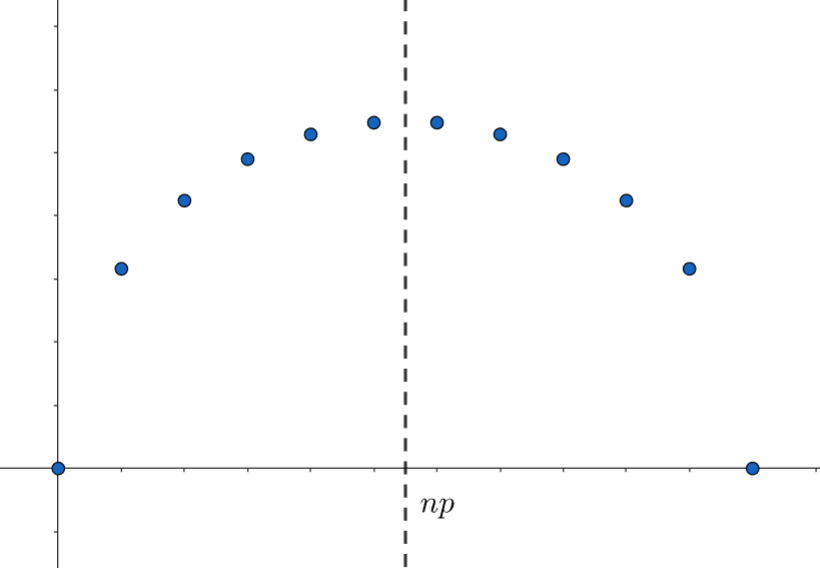
\includegraphics[width=6cm]{probtheory/images/probtheory_2024_09_24_1}
    \end{center}

    При увеличении числа $n$ точки превращаются в кривую Гаусса

    \begin{center}
        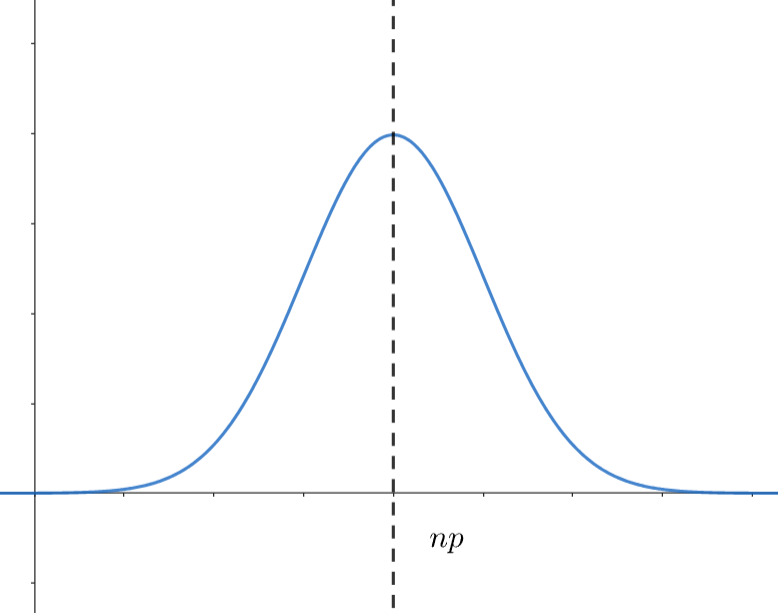
\includegraphics[width=6cm]{probtheory/images/probtheory_2024_09_24_2}
    \end{center}

    При увеличении числа испытаний $n$ формула Бернулли вырождается в следующие асимптотические формы (применяем, если требуется найти вероятность точного числа успеха)

    1) локальная формула Муавра-Лапласа

    $p_n(k) \underset{n \to \infty}{\longrightarrow} \frac{1}{\sqrt{npq}} \varphi(x)$, где $\varphi(x) = \frac{1}{\sqrt{2\pi}} e^{-\frac{x^2}{2}}$ - функция гаусса

    $x = \frac{k - np}{\sqrt{npq}}$

    Свойства $\varphi(x)$:

    1. $\varphi(x) = \varphi(-x)$ - функция четная

    2. при $x > 5 \quad \varphi(x) \approx 0$

    2) Интегральная формула Муавра-Лапласа (если требуется найти вероятность того, что число успехов в данном диапазоне)

    $p_n(k_1 \leq k \leq k_2) \underset{n \to \infty}{\longrightarrow} \Phi(x_2) - \Phi(x_1)$, где $\Phi(x) = \frac{1}{\sqrt{2\pi}} \int_0^x e^{-\frac{z^2}{2}} dz$ - функция Лапласа

    $x_1 = \frac{k_1 - np}{\sqrt{npq}}$ - отклонение от левой границы, $x_2 = \frac{k_2 - np}{\sqrt{npq}}$ - отклонение от правой

    Свойства $\Phi(x)$

    1. $\Phi(-x) = -\Phi(x)$ - функция нечетная

    2. при $x > 5 \quad \Phi(x) \approx 0.5$

    \Nota Эти формулы обычно можно применять при $n \geq 100$ и $0.1 \leq p \leq 0.9$

    \Nota В некоторых источниках под функцией Лапласа подразумевают другую функцию: $F_0(x) = \frac{1}{\sqrt{2\pi}} \int_{-\infty}^x e^{-\frac{t^2}{2}}dt$ - стандартное отклонение. Эта функция
    отличается от $F_0 = \frac{1}{\sqrt{2\pi}} \int_{-\infty}^0 e^{-\frac{t^2}{2}}dt + \Phi(x) = \frac{1}{2} + \Phi(x)$

    Так как $\int_{-\infty}^{\infty} e^{-x^2} dx = \sqrt{\pi}$ - интеграл Пуасона

    \Ex Вероятность попадания стрелка в цель $0.8$, стрелок сделал 400 выстрелов. Найти вероятность того, что:

    а) произошло ровно 330 попаданий

    б) произошло от 312 до 336 попаданий

    а) $x = \frac{k - np}{\sqrt{npq}} = \frac{330 - 400 \cdot 0.8}{\sqrt{400 \cdot 0.8 \cdot 0.2}} = \frac{330 - 320}{8} = 1.25$

    $p_{400}(330) \approx \frac{1}{\sqrt{npq}} \varphi(1.25) = \frac{1}{8} \varphi(1.25) \approx \frac{1}{8} \cdot 0.1826 \approx 0.0228$

    б) $x_1 = \frac{312 - 320}{8} = -1$, $x_2 = \frac{336 - 320}{8} = 2$

    $p_{400}(312 \leq k \leq 336) \approx \Phi(2) - \Phi(-1) = \Phi(2) + \Phi(1) \approx 0.4772 + 0.3413 = 0.8185$

    \subsection{Статистическое понятие вероятности}

    Пусть проводим $n$ реальных экспериментов, $n_A$ - число появления события $A$, $\frac{n_A}{n}$ - относительная частота события $A$.

    Эксперименты с монетой показали, что при больших $n$, $\frac{n_A}{n} \approx p(A)$ - явление стабилизации

    Вероятность отклонения относительной частоты от вероятности события

    $n$ - число испытаний, $p = p(A), \frac{n_A}{n}$ - экспериментальная частота

    $p\left(|\frac{n_A}{n} - p| \leq \varepsilon\right) = p\left(-\varepsilon \leq \frac{n_A}{n} - p \leq \varepsilon\right) = p(-n\varepsilon \leq n_A - np \leq n\varepsilon) = p(np - n\varepsilon \leq n_A \leq n\varepsilon + np) \underset{n \to \infty}{\longrightarrow}$ [по интегральной формуле Лапласа] $\underset{n \to \infty}{\longrightarrow} \Phi\left(\frac{n\varepsilon}{\sqrt{npq}}\right) - \Phi\left(-\frac{n\varepsilon}{\sqrt{npq}}\right)$

    $ = \Phi\left(\frac{\sqrt{n}\varepsilon}{\sqrt{pq}}\right) - \Phi\left(-\frac{\sqrt{n}\varepsilon}{\sqrt{pq}}\right)$

    $ = 2\Phi\left(\frac{\sqrt{n}\varepsilon}{\sqrt{pq}}\right)$

    Итак, получили, что нужная нам вероятность $p\left(|\frac{n_A}{n} - p| \leq \varepsilon\right) \approx 2\Phi\left(\frac{\sqrt{n}\varepsilon}{\sqrt{pq}}\right)$

    \subsection{Закон больших чисел Бернулли}

    Итак, $p\left(|\frac{n_A}{n} - p| \leq \varepsilon\right) \underset{n \to \infty}{\longrightarrow} 2 \Phi\left(\frac{\varepsilon}{\sqrt{pq}}\sqrt{n}\right)$

    при $n \to \infty, \sqrt{n} \to \infty, \frac{\varepsilon}{\sqrt{pq}} \sqrt{n} \to \infty, \Phi\left(\frac{\varepsilon}{\sqrt{pq}}\sqrt{n}\right) \to 0.5, p\left(|\frac{n_A}{n} - p| \leq \varepsilon\right) \to 2 \cdot 0.5 = 1$ - закон больших чисел показывает, что вероятность попадания относительной частоты в $\varepsilon$-трубу вероятность события приближается к 1

    $\lim_{n \to \infty} p\left(|\frac{n_A}{n} - p| \leq \varepsilon\right) = 1$ или $\frac{n_A}{n} \underset{n \to \infty}{\longrightarrow} p$ - сходимость по вероятности

    \Ex Для оценки доли $p$ курящих людей берется выборка объема $n$, и делается оценка доли курящих людей по формуле $p^* = \frac{n_A}{n}$.
    Каким должен быть объем $n$, чтобы с вероятностью $\gamma = 0.95$ данная оценка отличалась от истинного значения не более, чем на $\varepsilon = 0.01$

    По формуле вероятности отклонения частоты от вероятности $p(|p^* - p| \leq \varepsilon) = p\left(|\frac{n_A}{n} - p| \leq \varepsilon\right) \approx 2\Phi\left(\frac{\varepsilon}{\sqrt{pq}}\sqrt{n}\right) = 0.95$

    $\Phi\left(\frac{\varepsilon}{\sqrt{pq}}\sqrt{n}\right) = 0.475$

    $\frac{\varepsilon}{\sqrt{pq}}\sqrt{n} = 1.96$

    $\frac{1}{\sqrt{pq}}\sqrt{n} = 196$

    $\frac{n}{pq} = 38416$

    $n \geq 38416 pq$

    В самое худшей ситуации $pq \leq 0.5^2 = \frac{1}{4}$

    $n \geq \frac{38416}{4} = 9604$
% end probtheory_2024_09_24.tex

% begin probtheory_2024_10_01.tex

    \section{Лекция 5}

    \subsection{Схема испытаний и соответствующее распределение}

    Введем обозначения:

    $n$ - число испытаний

    $p$ - вероятность успеха при одном испытании

    $q = 1 - p$ - вероятность неудачи

    \subsubsection{I. Схема Бернулли}

    $\letsymbol v_n$ - число успехов в серии из $n$ испытаний

    $P_n(v_n = k) = C^k_n p^k q^{n - k}, \quad\quad k = 0, 1, \dots, n$

    \Def Соответствие $k \rightarrow C^k_n p^k q^{n - k}, \quad k = 0, \dots, n$ называется биномиальным распределением
    (обозначается $B_{n,p}$ или $B(n, p)$)

    \subsubsection{II. Схема до первого успешного испытания}

    Пусть проводится бесконечная серия испытаний, которая заканчивается после первого успешного испытания
    под номером $\tau$

    \begin{MyTheorem}
        \Ths $P(\tau = k) = q^{k - 1} p, \quad\quad k = 1, 2, \dots$
    \end{MyTheorem}

    \begin{MyProof}
        $\Box$

        $P(\tau = k) = P(\underset{k - 1}{\underbrace{\text{Н}\dots\text{Н}}}\text{У}) = q^{k - 1}p$

        $\Box$
    \end{MyProof}

    \Def Соответствие $k \rightarrow q^{k - 1} p, k \in \Natural$ называется геометрическим
    распределение вероятности (обозначается $G_p$ или $G(p)$)

    \Nota Геометрическое распределение обладает свойством \enqoute{нестарения} или свойством отсутствия
    последействия

    \begin{MyTheorem}
        \Ths $\letsymbol P(\tau = k) = q^{k - 1} p, k \in \Natural$. Тогда $\forall n, k \geq 0 \quad P(\tau > n + k \ | \ \tau > n) = P(\tau > k)$
    \end{MyTheorem}

    \begin{MyProof}
        $\Box$

        Заметим, что $P(\tau > m) = q^m$, первые $m$ - неудачи

        $P(\tau > n + k | \tau > n) = \frac{P(\tau > n + k, \tau > n)}{P(\tau > n)} = \frac{P(\tau > n + k)}{P(\tau > n)} = \frac{q^{n + k}}{q^n} = q^k$

        $\Box$
    \end{MyProof}

    \Nota $P(\tau = n + k \ | \ \tau > n) = p(\tau = k)$ - \Lab доказать

    \subsubsection{III. Схема испытаний с несколькими исходами}

    Пусть при $n$ независимых испытаний могут произойти $m$ исходов (несовместных)

    $p_i$ - вероятность $i$-ого исхода при одном испытании

    \begin{MyTheorem}
        \Ths Вероятность того, что при $n$ испытаниях первый исход появится $n_1$ раз, второй - $n_2$ раз, $m$-ый - $n_m$ ($\sum_{i = 1}^m n_i = n$)
        равно

        $P_n(n_1, n_2, \dots, n_m) = \frac{n!}{n_1! n_2! \dots n_m!} p_1^{n_1} p_2^{n_2} \dots p_m^{n_m}$
    \end{MyTheorem}

    При $m = 2$ получаем формулу Бернулли

    \begin{MyProof}
        $\Box$

        Рассмотрим следующий благоприятный исход, обозначим $A_1$

        $A_1 = \underset{n_1}{\underbrace{11\dots1}}\underset{n_2}{\underbrace{22\dots2}}\dots\underset{n_m}{\underbrace{mm\dots m}}$

        $p(A_1) = p_1^{n_1} p_2^{n_2} \dots p_m^{n_m}$

        Все остальные благоприятные исходы имеют ту же вероятность и отличаются лишь расположением $i$-ых исходов на $n$ позициях,
        получаем мультиномиальную теорему: $\frac{n!}{n_1! n_2! \dots n_m!}$

        В итоге получаем требуемую формулу

        $\Box$
    \end{MyProof}

    \Ex Два одинаковых сильных шахматиста играют шесть партий

    Вероятность ничьи в партии - $0.5$. Какова вероятность того, что второй игрок выиграет две партии, а еще три сведет к ничьей

    1-ый исход - выиграл 1 игрок

    2-ой исход - выиграл 2 игрок

    3-ий исход - ничья

    $n = 6; \quad p_3 = 0.5; \quad p_1 = p_2 = \frac{1 - p_3}{2} = 0.25$

    $P_6(1; 2; 3) = \frac{6!}{1!2!3!} \left(\frac{1}{4}\right)^1 \left(\frac{1}{4}\right)^2 \left(\frac{1}{2}\right)^3 = \frac{4 \cdot 5 \cdot 6}{2} \frac{1}{2^9} \approx 0.12$

    \subsubsection{IV. Урновая схема}

    В урне $N$ шаров, из которых $K$ шаров белые, $N - K$ - черные

    Из урны вынимаем (без учета порядка) $n$ шаров. Найти вероятность, что из них $k$ белых

    а) Схема с возвратом (после каждого раза кладем шар обратно). В этом случае вероятность вынуть белый шар одинакова и
    равна $\frac{K}{N}$. Получаем схему Бернулли: $P_n(k) = C^k_n \left(\frac{K}{N}\right)^k \left(1 - \frac{K}{N}\right)^{n - k}$

    б) Схема без возврата - вынутый шар мы выбрасываем

    $P_{N, K} (n, k) = \frac{C^k_K C^{n - k}_{N - K}}{C^n_N}$

    \Def Соответствие $k \rightarrow \frac{C^k_K C^{n - k}_{N - K}}{C^n_N}, k = 0, \dots, n$ называется гипергеометрическим
    распределением

    \Nota Если $K, N \to \infty$ так, что $\frac{K}{N} \approx p$ (не меняется), а $n$ и $k$ зафиксировать, то после выбора
    $n$ шаров пропорции состава шаров не сильно изменятся, поэтому логично предположить, что гипергеометрическое распределение
    будет сходиться к биномиальному

    \begin{MyTheorem}
        \Ths Если $K, N \to \infty$ таким образом, что $\frac{K}{N} \to p \in (0;1)$, а $n$ и $0 \leq k \leq n$ фиксированы, то
        вероятность при гипергеометрическом распределении будет стремиться к биномиальному:

        $P_{N,K} (n, k) = \frac{C^k_K C^{n - k}_{N - K}}{C^n_N} \rightarrow C^k_n \left(\frac{K}{N}\right)^k \left(1 - \frac{K}{N}\right)^{n - k}$
    \end{MyTheorem}

    Воспользуемся леммой: $C^k_n \sim \frac{n^k}{k!}$ при $n \to \infty$ и фиксированном $k$

    Доказательство леммы: $C_n^k = \frac{n!}{k!(n - k)!} = \frac{n(n - 1) \dots (n - k + 1)}{n^k} \frac{n^k}{k!} = 1 \left(1 - \frac{1}{n}\right) \dots \left(1 - \frac{k - 1}{n}\right) \frac{n^k}{k!} \sim \frac{n^k}{k!}$

    \begin{MyProof}
        $\Box$

        $P_{N,K} (n, k) = \frac{C^k_K C_{N - K}^{n - k}}{C^n_N} \sim \frac{K^k}{k!} \frac{(N - K)^{n - k}}{N^n} \frac{n!}{N^n} =
        \frac{n!}{k!} \frac{(N - K)^{n - k}}{N^n} \frac{K^k}{N^n} = C^k_n \left(\frac{K}{N}\right)^k \left(1 - \frac{K}{N}\right)^{n - k} \to C^k_n \left(\frac{K}{N}\right)^k \left(1 - \frac{K}{N}\right)^{n - k} $

        $\Box$
    \end{MyProof}

    \subsubsection{V. Схема Пуассона. Теорема Пуассона для схемы Бернулли}

    \Nota Если вероятность успеха $p$ в схеме Бернулли мала или близка к 1, то предельная формула Лапласа при недостаточно большом
    числе испытаний дает достаточно большую погрешность. В этой ситуации следует использовать формулу Пуасоона (формула редких событий)

    Схема: вероятность числа успеха при одном испытании $p_n$ зависит от числа испытаний $n$, причем таким образом, что $n p_n \approx \lambda = const$

    $\lambda$ - интенсивность появления редких событий в единицу времени в потоке испытаний

    \begin{MyTheorem}
        \ThNs{1} (формула Пуассона) Пусть $n \to \infty, p_n \to 0$ таким образом, что $n p_n \to \lambda = const > 0$

        Тогда вероятность $k$ успехов при $n$ испытаниях: $P_n(k) = C^k_n p_n^k (1 - p_n)^{n - k} \underset{n \to \infty}{\rightarrow} = \frac{\lambda^k}{k!} e^{-\lambda}$
    \end{MyTheorem}

    \begin{MyProof}
        $\Box$

        Обозначим $\lambda_n = n p_n$. Тогда $p_n = \frac{\lambda_n}{n}$ и

        $P_n(k) = C^k_n \left(\frac{\lambda_n}{n}\right)^k \left(1 - \frac{\lambda_n}{n}\right)^{n - k} \underset{n \to \infty}{\rightarrow} \frac{n^k}{k!} \frac{\lambda^k_n}{n^k} \left(1 - \frac{\lambda_n}{n}\right)^n \cancelto{1}{\left(1 - \frac{\lambda_n}{n}\right)^{-k}}
        \underset{n \to \infty}{\rightarrow} \frac{\lambda_n^k}{k!} \left(1 - \frac{\lambda_n}{n}\right) = \frac{\lambda_n^k}{k!} \left(\left(1 - \frac{\lambda_n}{n}\right)^{-\frac{n}{\lambda_n}}\right)^{-\frac{\lambda_n}{n}n} \underset{n \to \infty}{\rightarrow} \frac{\lambda_n^k}{k!} e^{-\lambda_n} \underset{n \to \infty}{\rightarrow} \frac{\lambda^k}{k!} e^{-\lambda}$

        $\Box$
    \end{MyProof}

    \begin{MyTheorem}
        \ThNs{2} (оценка погрешности в формуле Пуассона) Пусть $v_n$ - число успехов при $n$ испытаниях в схеме Бернулли

        $p$ - вероятность успеха при одном испытании, $\lambda = np$, $A \subset \{0, 1, \dots, n\}$ - произвольное подмножество чисел

        Тогда $|P_n (v_n \in A) - \sum_{k \in A} \frac{\lambda^k}{k!} e^{-\lambda}| \leq \min (p, np^2) = \min (p, p\lambda)$

        (без доказательства)
    \end{MyTheorem}

    \Def Соответствие $k \to \frac{\lambda^k}{k!} e^{-\lambda}, k = 0, 1, \dots$ называется распределением Пуассона
    с параметром $\lambda > 0$ (обозначается $\Pi_\lambda$)

    \Ex Прибор состоит из 1000 элементов, вероятность отказа каждого элемента равна $0.001$. Какова вероятность отказа больше двух элементов

    $P_n(k) \approx \frac{\lambda^k}{k!} e^{-\lambda}$

    $n = 1000, p = 0.001, \lambda = 1$

    $P_n(k > 2) = 1 - P_n (k \leq 2) = 1 - P(0) - P(1) - P(2) \approx 1 - \left(\frac{1^0}{0!} e^{-1} + \frac{1^1}{1!} e^{-1} + \frac{1^2}{2!} e^{-1}\right) =
    1 - \left(1 + 1 + \frac{1}{2}\right) e^{-1} \approx 0.0803$
% end probtheory_2024_10_01.tex

% begin probtheory_2024_10_08.tex

    \section{Лекция 6}

    \subsection{Случайные величины}

    Примеры случайных величин:

    \ExN{1} Бросаем кость, может выпасть 6 граней, здесь случайная величина $\xi$ - число выпавших очков

    \ExNs{2} $\xi$ - время работы микросхемы, в этом случае время может быть:

    а) дискретным - $\xi \in \{0, 1, 2, \dots\}$

    б) непрерывным - $\xi \in [0; \infty)$

    \ExNs{3} Температура за окном: $\xi \in (-50, +50)$

    \Def На вероятностном пространстве $(\Omega, \mathcal{F}, p)$ функция $\xi \ : \ \Omega \to \Real$ называется
    $\mathcal{F}$-измеримой, если $\forall x \in \Real \ \{\omega \in \Omega \ | \ \xi(\omega) < x\} \in \mathcal{F}$
    (то есть $\xi^{-1}(y) \in \mathcal{F}$, где $y \in (-\infty; x)$)

    \Def Случайной величиной, заданной на вероятностном пространстве $(\Omega, \mathcal{F}, p)$, называется
    $\mathcal{F}$-измеримая функция $\xi \ : \Omega \to \Real$, которая сопоставляет каждому элементарному исходу \
    некоторое вещественное число

    \Nota Не все функции являются $\mathcal{F}$-измеримыми

    \Exs Кость: $\Omega = \{1, 2, 3, 4, 5, 6\}; \mathcal{F} = \{\emptyset, \Omega, \{2, 4, 6\}, \{1, 3, 5\}\}$

    Пусть $\xi(\omega) = i$ - число выпавших очков. Тогда при $x = 4: \{\omega \in \Omega \ | \ \xi (\omega) < 4\} = \{1, 2, 3\} \notin \mathcal{F} \Longrightarrow$ случайная величина не является $\mathcal{F}$-измеримой

    В данном случае следует сделать $\xi$ таким, что $\xi(2) = \xi(4) = \xi(6) = 1$, $\xi(1) = \xi(3) = \xi(5) = 0$

    \Nota Смысл измеримости: если задана случайная величина $\xi$, то мы можем задать вероятность попадания случайной
    величины в интервал $(-\infty; x)$: $p(\xi \in (-\infty; x)) = p(\{\omega \in \Omega \ | \ \xi(\omega) < x\})$

    А из интервалов $(-\infty; x)$ с помощью операций пересечения, объединения и дополнения можно получить все другие
    интервалы (включая точки) и также приписать им вероятности

    Из матанализа известно, что мера из интервалов однозначно продолжается до меры на всей Борелевской $\sigma$-алгебры на $\Real$
    и, таким образом, с помощью случайной величины каждому Борелевскому множеству $B$ также приписывается вероятность $p(\xi \in B)$

    Итак, пусть $\xi$ задана на вероятностном пространстве $(\Omega, \mathcal{F}, p)$, с помощью нее получаем новой вероятностное
    пространство $(\Real, \mathcal{B}(\Real), p_\xi)$

    Получая новое вероятностное пространство, мы упрощаем и формализуем работу, так как можем не учитывать природу и структуру исходного пространства

    \Def Функция $p(B), B \in \mathcal{B}(\Real)$, ставящая в соответствие каждому Борелевскому множеству вероятность,
    называется распределением случайной величины $\xi$

    \subsection{Основные типы распределения}

    \begin{enumerate}[label=\alph*) ]
        \item Дискретное

        \item Абсолютно непрерывное

        \item Сингулярное

        \item Смешанное
    \end{enumerate}

    \subsection{Дискретная случайная величина}

    \Def Случайная величина $\xi$ имеет дискретное рапределение, если она принимает не более, чем счетное число значений.
    То есть существует конечный или счетный набор чисел $\{x_1, x_2, \dots, x_n, \dots\}$ такой, что $p(\xi = x_i) = p_i > 0$ и $\sum_{i = 0}^\infty p_i = 1$

    Таким образом, дискретная случайная величина (ДСВ) задается законом распределения:

    доска

    \smallvspace

    \begin{tabular}{c|c|c|c|c|cl}
        $\xi$ & $x_1$ & $x_1$ & \dots & $x_n$ & \dots & \text{\qquad   - значения случайной величины} \\
        \cline{1-6}
        $p$   & $p_1$ & $p_1$ & \dots & $p_n$ & \dots & \text{\qquad   - вероятности этих значений}
    \end{tabular}

    \smallvspace


    ($\sum_{i = 0}^\infty p_i = 1$ - условие нормировки)

    \ExN{1} кость, $\xi(\omega) = i$ - число выпавших очков

    \smallvspace

    %nodisplay

    \begin{tabular}{c|c|c|c|c|c|c}
        $\xi$ & $1$           & $2$           & $3$           & $4$           & $5$           & $6$           \\
        \hline
        $p$   & $\frac{1}{6}$ & $\frac{1}{6}$ & $\frac{1}{6}$ & $\frac{1}{6}$ & $\frac{1}{6}$ & $\frac{1}{6}$
    \end{tabular}

    %yesdisplay

    \smallvspace

    \ExNs{2} все распределения из предыдущих лекций (биномиальное, геометрическое, гипергеометрическое, Пуассона)

    \ExNs{3} индикатор события $A$: $I_A (\omega) = \begin{cases}
                                                        0, \quad \omega \notin A \text{ - событие } A \text{ не происходит} \\ 1, \quad \omega \in A \text{ - событие } A \text{ происходит}
    \end{cases}$

    \subsection{Числовые характеристики дискретных случайных величин}

    \subsubsection{I. Математическое ожидание (среднее значение, полезность)}

    \Defs Математическим ожиданием $E\xi$ случайной величины $\xi$ называется число

    \[ E\xi = \sum_{i = 1}^\infty x_i p_i \]

    при условии, что данный ряд сходится абсолютно

    \Nota Если $E\xi = \sum_{i = 1}^\infty x_i p_i = \infty$, то говорят, что матожидание не существует

    При условной сходимости ряда при перестановке членов сумма изменяется, поэтому необходима абсолютная

    \textbf{Физический смысл}: Среднее значение - число, вокруг которого группируются значения случайной величины, центр тяжести точек $x_i$ с весами $p_i$

    \textbf{Статистический смысл}: среднее арифметическое наблюдаемых значений случайной величины при
    большом числе реальных экспериментов

    \subsubsection{II. Дисперсия}

    \Defs Дисперсией $D\xi$ случайной величины $\xi$ называют среднее квадратов ее отклонения от математического ожидания:

    $D\xi = E (\xi - E\xi)^2$ или $D\xi = \sum_{i = 0}^\infty (x_i - E\xi)^2 p_i$ при условии, что данный ряд сходится

    В противном случае говорится, что дисперсии не существует

    \Nota Дисперсию обычно удобно считать по формуле $D\xi = E\xi^2 - (E\xi)^2 = \sum_{i = 1}^n x^2_i p_i - E\xi^2$

    \textbf{Смысл} - квадрат среднего разброса (рассеивания) значения случайной величины относительно ее математического
    ожидания

    \subsubsection{III. Среднее квадратическое отклонение}

    \Defs Среднее квадратическое отклонение (СКО) $\sigma_\xi$ называется величина $\sigma_\xi = \sqrt{D\xi}$

    \textbf{Смысл} - средний разброс

    \ExN{1} Кость

    \smallvspace

    %nodisplay

    \begin{tabular}{c|c|c|c|c|c|c}
        $\xi$ & $1$           & $2$           & $3$           & $4$           & $5$           & $6$           \\
        \hline
        $p$   & $\frac{1}{6}$ & $\frac{1}{6}$ & $\frac{1}{6}$ & $\frac{1}{6}$ & $\frac{1}{6}$ & $\frac{1}{6}$
    \end{tabular}

    %yesdisplay

    $E\xi = \sum_{i = 1}^6 x_i p_i = 3.5$ (в данном случае ср. арифм.)

    $D\xi = \sum_{i = 1}^6 (x_i - E\xi)^2 p_i = 1^2 \cdot \frac{1}{6} + 2^2 \cdot \frac{1}{6} + 3^2 \cdot \frac{1}{6} + 4^2 \cdot \frac{1}{6} + 5^2 \cdot \frac{1}{6} + 6^2 \cdot \frac{1}{6} - 3.5^2 = \frac{35}{12} $

    $\sigma_\xi = \sqrt{D\xi} \approx 1.79$

    \ExN{2} Индикатор события $A$: $I_A (\omega) = \begin{cases}
                                                       0, \omega \notin A \text{ - событие } A \text{ не происходит} \\ 1, \omega \in A \text{ - событие } A \text{ происходит}
    \end{cases}$

    \begin{tabular}{c|c|c}
        $\xi$ & $0$        & $1$    \\
        \hline
        $p$   & $1 - P(A)$ & $P(A)$
    \end{tabular}

    $E\xi = 0 \cdot (1 - P(A)) + 1 \cdot P(A) = P(A)$

    $D\xi = 0^2 \cdot (1 - P(A)) + 1^2 P(A) - P(A)^2 = P(A) (1 - P(A)) = pq$

    $\sigma_\xi = \sqrt{pq}$

    \subsection{Свойства матожидания и дисперсии}

    \begin{MyTheorem}
        \ThNs{1} Случайная величина $\xi$ имеет вырожденное распределение, если $\xi(\omega) = \mathrm{const} \ \ \forall \omega \in \Omega$

        \begin{tabular}{c|c}
            $\xi$ & $C$ \\
            \hline
            $p$   & $1$
        \end{tabular}

        $E\xi = C \qquad D\xi = 0$
    \end{MyTheorem}

    \begin{MyTheorem}
        \ThNs{2} Свойство сдвига: $E(\xi + C) = E\xi + C; D (\xi + C) = D\xi$
    \end{MyTheorem}

    \begin{MyTheorem}
        \ThNs{3} Свойство растяжения:

        $E(C\xi) = CE\xi$

        $D(C\xi) = C^2 D\xi$
    \end{MyTheorem}

    \Lab 2-3 доказать

    \begin{MyTheorem}
        \ThNs{4} $E(\xi + \eta) = E\xi + E\eta$ (из третьего свойства матожидание - линейная функция)
    \end{MyTheorem}

    \begin{MyProof}
        $\Box$

        $\letsymbol x_i, y_i$ - значения случайных величин $\xi, \eta$, а $p_i$ и $q_i$ - их соответствующие вероятности

        $E(\xi + \eta) = \sum_{i, j} (x_i + y_j) p(\xi = x_i \text{ и } \eta = y_j) = \sum_i x_i \sum_j p(\xi = x_i \text{ и } \eta = y_j) + \sum_j y_j \sum_i p(\xi = x_i \text{ и } \eta = y_j) =
        \sum_i x_i p(\xi = x_i) + \sum_j y_j p(\eta = y_j) = E\xi + E\eta$

        $\Box$
    \end{MyProof}

    \Def Дискретные случайные величины $\xi$ и $\eta$ независимы, если $p(\xi = x_i, \eta = y_i) = p(\xi = x_i) \cdot p(\eta = y_i) \ \forall i, j$

    То есть случайные величины принимают свои величины независимо друг от друга

    \begin{MyTheorem}
        \ThNs{5} Если случайные свойства $\xi$ и $\eta$ независимы, то $E(\xi \eta) = E\xi \cdot E\eta$; обратное неверно
    \end{MyTheorem}

    \begin{MyProof}
        $\Box$

        $E(\xi\eta) = \sum_{i, j} x_i y_i p(\xi = x_i, \eta = y_j) = \sum_i x_i \sum_j y_j p(\xi = x_i, \eta = y_j) =
        \sum_i x_i \sum_j y_j p(\xi = x_i) p(\eta = y_j) = \sum_i x_i p(\xi = x_i) \sum_j y_j p(\eta = y_j) = E\xi \cdot E\eta$

        $\Box$
    \end{MyProof}

    \begin{MyTheorem}
        \ThNs{6} $D\xi = E\xi^2 - (E\xi)^2$
    \end{MyTheorem}

    \begin{MyProof}
        $\Box$

        $D\xi = E(\xi - E\xi)^2 = E(\xi^2 - 2\xi E\xi + (E\xi)^2) = E\xi^2 - 2E\xi E\xi + E((E\xi)^2) =
        E\xi^2 - 2(E\xi)^2 + (E\xi)^2 = E\xi^2 - (E\xi)^2$

        $\Box$
    \end{MyProof}

    \Def $D(\xi + \eta) = D\xi + D\eta + 2\mathrm{cov} (\xi, \eta)$,
    где $\mathrm{cov}(\xi, \eta) = E(\xi\eta) - E\xi E\eta$ - ковариация случайных величин (равна 0 при независимых величинах) - индикатор наличия связи между случайными величинами

    \begin{MyProof}
        $\Box$

    $D(\xi + \eta) = E(\xi + \eta)^2 - (E(\xi + \eta))^2 = E\xi^2 + 2E\xi E\eta + E\eta^2 - (E\xi + E\eta)^2 =
    E\xi^2 + E\eta^2 + 2E(\xi\eta) - (E\xi)^2 - (E\eta)^2 - 2E\xi E\eta = D\xi + D\eta + 2\mathrm{cov}(\xi, \eta)$

        $\Box$
    \end{MyProof}


    \begin{MyTheorem}
        \ThNs{7} Если случайные величины $\xi$ и $\eta$ независимы, то $D(\xi + \eta) = D\xi + D\eta$
    \end{MyTheorem}

    \begin{MyProof}
        $\Box$

        Если $\xi$ и $\eta$ независимы, то $\mathrm{cov}(\xi, \eta) = 0$ и $D(\xi + \eta) = D\xi + D\eta$

        $\Box$
    \end{MyProof}

    \begin{MyTheorem}
        \ThNs{8} Общая формула дисперсии суммы: $D(\xi_1 + \xi_2 + \dots + \xi_n) = \sum_{i = 1}^n D \xi_i + 2\sum_{i, j (i \neq j)} \mathrm{cov} (\xi_i, \xi_j)$
    \end{MyTheorem}

    \subsection{Другие числовые характеристики}

    Моменты старших порядков

    а) $m_k = E\xi^k$ - момент $k$-ого порядка случайной величины $\xi$

    б) $\mu_k = E(\xi - E\xi)^k$ - центральный момент $k$-ого порядка

    $E\xi = m_1$ - момент первого порядка

    $E\xi^2 = m_2$ - момент второго порядка

    $D\xi = E(\xi - E\xi)^2$ - центральный момент второго порядка

    \Nota Центральные моменты можно выразить через обычный момент:

    $\mu_2 = D\xi = E\xi^2 - (E\xi)^2 = m_2^2 - m_1^2$

    $\mu_3 = m_3 - 3m_2 m_1 + 2m^3$

    $\mu_4 = m_4 - 4m_3 m_2 + 6m_2 m_1^2 - 3m_1^4$

    \Ex Разберем \hyperlink{buffonsproblem}{задачу Бюффона} с точки зрения матожидания (для простоты $l$ - ширина доски): пусть $p(A)$ - пересечет стык,
    $\xi = I_A$ - число пересечений. Тогда матожидание $E\xi = E I_A = P(A)$

    Заметим, что при изменении длины иглы с $l$ до $2l$ матожидание пересекаемых стыков увеличивается
    в два раза. Помимо этого можно составить из $k$ игл ломаную, матожидание стыков которой будет равно $kE\xi$

    Заметим, что такое работает и в обратную сторону: при уменьшении иглы в $k$ раз матожидание равно $\frac{E\xi}{k}$

    Теперь сделаем замкнутый многоугольник из игл, получим, что матожидание в таком случае $P\frac{E\xi}{l}$, где $P$ - периметр

    В пределе строим круг диаметра $l$ - он всегда пересечет линии стыка 2 раза, значит матожидание $E_o = P_o\frac{E\xi}{l} = 2$

    Длина окружность $P_o = \pi l$, получаем $E\xi = \frac{2l}{P_o} = \frac{2l}{\pi l} = \frac{2}{\pi}$
% end probtheory_2024_10_08.tex

% begin probtheory_2024_10_15.tex

    \section{Лекция 7}

    \subsection{Стандартное дискретное распределение}

    \subsubsection{I. Распределение Бернулли}

    Распределение Бернулли $B_p$ (с параметром $0 < p < 1$)

    $\xi$ - число успехов при одном испытании, $p$ - вероятность успеха при одном испытании
    
    \smallvspace

    \begin{tabular}{c|c|c}
        $\xi$ & $0$        & $1$    \\
        \hline
        $p$   & $1 - P(A)$ & $P(A)$
    \end{tabular}

    \smallvspace

    Матожидание: $E\xi = p$

    Дисперсия: $D\xi = p(1 - p) = pq$

    \Ex Индикатор события $I_A \in B_p$ как раз имеет распределение Бернулли, где $p = P(A)$

    \subsubsection{II. Биномиальное распределение}

    Биномиальное распределение $B_{n,p}$ (с параметрами $n, p$)

    $\xi$ - число успехов в серии из $n$ испытаний, $p$ - вероятность успеха при одном испытании

    $p(\xi = k) = C^k_n p^k q^{n - k}, \ k = 0, 1, \dots, n \Longleftrightarrow \xi \in B_{n,p}$

    \smallvspace

    \begin{tabular}{c|c|c|c|c|c|c}
        $\xi$ & $0$        & $1$ & \dots & $k$ & \dots & $n$    \\
        \hline
        $p$   & $q^n$ & $n q^{n - 1} p$ & \dots & $C^k_n p^k q^{n - k}$ & \dots & $p_n$
    \end{tabular}

    \smallvspace

    Заметим, что $\xi = \xi_1 + \xi_2 + \dots + \xi_n$, где $\xi_i \in B_p$ - число успехов при $i$-ой испытании

    $E\xi_i = p; \quad D\xi = pq$

    $E\xi = E\xi_1 + \dots + E\xi_n = p + \dots + p = $ \fbox{$np$}

    $D\xi = D\xi_1 + \dots + D\xi_n = pq + \dots + pq = $ \fbox{$npq$}

    
    \subsubsection{III. Геометрическое распределение}

    Геометрическое распределение $G_p$ (с параметром $p$)

    $\xi$ - номер 1-ого успешного испытания в бесконечной серии

    $p(\xi = k) = q^{k - 1}p, \ k = 1, 2, 3, \dots \Longleftrightarrow \xi \in G_p$

    \smallvspace
    
    \begin{tabular}{c|c|c|c|c|c|c}
        $\xi$ & $1$ & $2$ & \dots & $k$ & \dots & $n$    \\
        \hline
        $p$   & $p$ & $qp$ & \dots & $q^{k - 1}p$ & \dots & $p_n$
    \end{tabular}

    \smallvspace

    Матожидание $E\xi = \sum_{k = 1}^\infty k p(\xi = k) = \sum_{k = 1}^\infty k q^{k - 1} p = p \sum_{k = 1}^\infty k q^{k - 1} = 
    p \sum_{k = 1}^\infty (q^k)^\prime = p \left(\sum_{k = 1}^\infty (q^k)\right)^\prime = p \left(\frac{1}{1 - q}\right)^\prime = 
    \frac{p}{p^2} = \frac{1}{p}$

    $E\xi^2 = \sum_{k = 1}^\infty k^2 q_{k - 1} p = p \sum_{k = 1}^\infty k(k - 1)q^{k - 1} = pq \sum_{k = 1}^\infty k(k - 1)q^{k - 2} + E\xi = 
    pq (\sum_{k = 1}^\infty q^k)^{\prime\prime} + \frac{1}{p} = pq \left(\frac{1}{1 - q}\right)^{\prime\prime} + \frac{1}{p} = 
    2pq \frac{1}{(1 - q)^3} + \frac{1}{p} = 2pq \frac{1}{p^3} + \frac{1}{p} = \frac{2q}{p^2} + \frac{1}{p}$
    
    $D\xi = E\xi^2 - (E\xi)^2 = \frac{2q}{p^2} + \frac{1}{p} - \frac{1}{p^2} = \frac{q}{p^2}$

    
    \subsubsection{IV. Распределение Пуассона}

    Распределение Пуассона $\Pi_\lambda$ (с параметром $\lambda > 0$)

    \Def Случайная величина $\xi$ имеет распределение Пуассона с параметром $\lambda > 0$, если $p(\xi = k) = \frac{\lambda^k}{k!}e^{-\lambda}, \ k = 0, 1, 2, \dots$

    \smallvspace

    \begin{tabular}{c|c|c|c|c|c|c}
        $\xi$ & $0$ & $1$ & \dots & $k$ & \dots & $n$    \\
        \hline
        $p$   & $e^{-\lambda}$ & $\lambda e^{-\lambda}$ & \dots & $\frac{\lambda^k}{k!}e^{-\lambda}$ & \dots & $p_n$
    \end{tabular}

    \smallvspace

    Покажем корректность определения - докажем, что сумма нижней строки равна 1:

    $\sum_{k = 0}^\infty p_k = \sum_{k = 0}^\infty \frac{\lambda^k}{k!} e^{-\lambda} = e^{-\lambda} \underset{\substack{\text{ряд Тейлора}\\ \text{для } e^x}}{\underbrace{\sum_{k = 0}^\infty \frac{\lambda_k}{k!}}} = e^{-\lambda} e^\lambda = 1$

    $E\xi = \sum_{k = 0}^\infty k \cdot \frac{\lambda^k}{k!}e^{-\lambda} = e^{-\lambda} \sum_{k = 0}^\infty \frac{\lambda^k}{(k - 1)!} = 
    \lambda e^{-\lambda} \sum_{k = 0}^\infty \frac{\lambda^{k - 1}}{(k - 1)!} = \lambda e^{-\lambda} e^\lambda = \lambda = np$

    
    $E\xi^2 = \sum_{k = 0}^\infty k^2 \cdot \frac{\lambda^k}{k!}e^{-\lambda} = e^{-\lambda} \sum_{k = 2}^\infty k(k - 1) \frac{\lambda^k}{k!} + 
    e^{-\lambda} \sum_{k = 1}^\infty k \frac{\lambda^k}{k!} = \lambda^2 e^{-\lambda} \sum_{k = 2}^\infty \frac{\lambda^{k - 2}}{(k - 2)!} + 
    \lambda e^{-\lambda} \sum_{k = 1}^\infty \frac{\lambda^{k - 1}}{(k - 1)!} = \lambda^2 e^{-\lambda} e^\lambda + \lambda e^{-\lambda} e^\lambda = \lambda^2 + \lambda$

    $D\xi = E\xi^2 - (E\xi)^2 = \lambda^2 + \lambda - \lambda^2 = \lambda$

    \clearpage

    \subsection{Задача о разорении игрока}

    Постановка задачи: играют 2 игрока, вероятность выигрыша первого игрока в одной игре равна $p$, $q = 1 - p$ - вероятность его проигрыша (выигрыш второго)

    В каждой игре разыгрывается 1 биткоин. Капитал первого игрока - $k$ биткоинов, $m - k$ биткоинов - капитал второго

    Найти вероятность разорения первого игрока

    Траектория капитала первого игрока будет выглядить как-то так:

    \begin{center}
        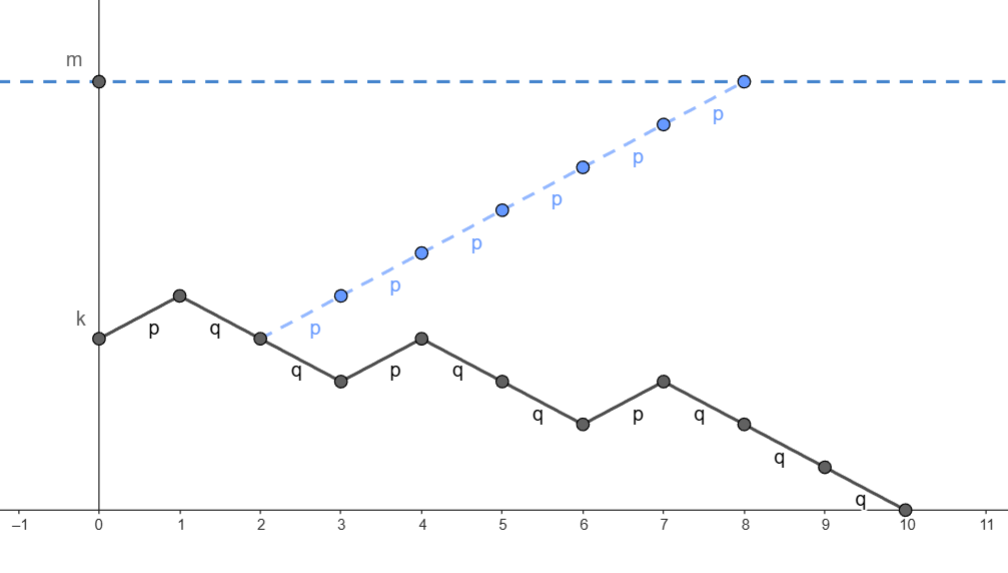
\includegraphics[height=7cm]{probtheory/images/probtheory_2024_10_15_1}
    \end{center}

    Пусть $r_k$ - интересующая нас вероятность разорение игрока при капитале $k$ (то есть достижения оси абсцисс на графике)

    $r_k = p \cdot r_{k + 1} + q r_{k - 1}$

    $pr_{k + 1} - r_k + (1 - p) r_{k - 1} = 0, \quad r_0 = 1, r_{m} = 0$

    $p\lambda^2 - \lambda + (1 - p) = 0$

    $D = 1 - 4p(1 - p) = 4p^2 - 4p + 1 = (2p - 1)^2$

    $\lambda_{1, 2} = \frac{1 \pm (2p - 1)}{2p}; \quad \lambda_1 = 1; \lambda_2 = \frac{2 - 2p}{2p} = \frac{q}{p}$

    Обозначим $\lambda = \frac{q}{p}$

    Рассмотрим два случая: 

    \begin{itemize}
        \item $p \neq \frac{1}{2}$

        Тогда общее решение: $r_k = C_1 \lambda_1^k + C_2 \lambda_2^k = C_1 + C_2 \lambda^k$

        Найдем частное решение:

        $\begin{cases}
            1 = C_1 + C_2 \\
            0 = C_1 + C_2 \lambda^m
        \end{cases} \Longleftrightarrow \begin{cases}
            C_1 = 1 - C_2 \\
            1 - C_2 + C_2 \lambda_m = 0
        \end{cases} \Longleftrightarrow \begin{cases}
            C_1 = 1 - C_2 \\
            C_2 (1 - \lambda_m) = 1
        \end{cases} \Longleftrightarrow \begin{cases}
            C_1 = 1 - \frac{1}{1 - \lambda^m} = \frac{-\lambda^m}{1 - \lambda^m} \\
            C_2 = \frac{1}{1 - \lambda^m}
        \end{cases}$

        $r_k = \frac{-\lambda^m}{1 - \lambda^m} + \frac{1}{1 - \lambda^m} \lambda^k = \frac{\lambda^k - \lambda^m}{1 - \lambda^m}$

        Посмотрим, что будет происходит при бесконечной игре (то есть когда $m \to \infty$ - капитал неограничен)

        1) $p < q$, то есть $\lambda > 1$. Тогда $\lambda^m \to \infty$, $r_k = \frac{\lambda^k - \lambda^m}{1 - \lambda^m} = \frac{\frac{\lambda^k}{\lambda_m} - 1}{\frac{1}{\lambda^m} - 1} \underset{n \to \infty}{\longrightarrow} 1$ - 
        то есть первый игрок гарантированно разорится

        2) $p > q$, то есть $\lambda < 1$. Тогда $\lambda^m \to 0$, $r_k = \frac{\lambda^k - \lambda^m}{1 - \lambda^m} \underset{n \to \infty}{\longrightarrow} \lambda^k$ - 
        то есть $r_k = \left(\frac{q}{p}\right)^k$

        \item $p = \frac{1}{2} \Longrightarrow D = 0$ 

        Тогда $\lambda_1 = \lambda_2 = 1$

        Общее решение: $r_k = C_1 \lambda^k + C_2 k \lambda_k = C_1 + C_2 k$

        Частное решение: 
        
        $\begin{cases}
            1 = C_1 \\
            0 = C_1 + C_2 m
        \end{cases} \Longleftrightarrow \begin{cases}
            1 = C_1 \\
            -1 = C_2 m
        \end{cases} \Longleftrightarrow \begin{cases}
            1 = C_1 \\
            C_2 = -\frac{1}{m}
        \end{cases}$

        $r_k = 1 - \frac{k}{m}$

        При бесконечной игре:

        $r_k = 1 - \frac{k}{m} \underset{m \to \infty}{\longrightarrow} 1$ - то есть при равной игре игрок неминуемо разорится 

    \end{itemize}

    \subsection{Случайное блуждание на прямой}

    Пусть в начальный момент времени находимся в начале координат. С вероятностью $p$ идем на единицу вправо, с вероятностью $q$ - влево

    При $p = \frac{1}{2}$ мы рано или поздно попадем в любую точку числовой прямой

    Можно привести аналогию с орлянкой: рано или поздно каждый игрок будет при сколь угодно большом выигрыше

    Посмотрим на орлянку как на распределение Бернулли:

    \smallvspace

    \begin{tabular}{c|c|c}
        $\xi$ & $-1$        & $1$    \\
        \hline
        $p$   & $\frac{1}{2}$ & $\frac{1}{2}$
    \end{tabular}

    \smallvspace

    $E\xi = 0; \quad D\xi = 1$

    Пусть $\xi$ - выигрыш первого после $n$ игр.

    $E\xi = \sum_{i = 1}^n E\xi_i = 0$

    $D\xi = \sum_{i = 1}^n D\xi_i = n$

    $\sigma_\xi = \sqrt{n}$ - среднее квадратическое отклонение

    Это означает, что при большом $n$ СКО поглотит всю числовую прямую

    $\frac{S_n}{n} \to E\xi$

    Закон больших чисел в этой ситуации говорит, что точка останется у 0, однако в то же время она может оказаться на любой точке на числовой прямой

    \Ex По $n$ конвертам случайным образом раскладывается $m$ писем. Случайная величина $\xi$ - число писем в своих конвертах

    $\letsymbol A_i$ - число $i$ письма в своем конверте, $\xi_i = I_A = \begin{cases}0, \quad i\text{-ое письмо в не своем конверте} \\ 1, \quad i\text{-ое письмо в своем конверте} \end{cases}$

    $\xi = \sum_{i = 1}^n \xi_i$

    $E\xi_i = P(A_i) = \frac{1}{n}$

    $D\xi_i = pq = \frac{1}{n} (1 - \frac{1}{n}) = \frac{n - 1}{n^2}$

    $E\xi = \sum_{i = 1}^n E\xi_i = 1 \frac{1}{n} = 1$ - в среднем будет одно письмо в своем конверте

    $D\xi = D(\xi_1 + \dots + \xi_n) = \sum_{i = 1}^n D\xi_i + 2\sum_{i < j} \mathrm{cov} (\xi_i, \xi_j)$

    Найдем ковариацию:

    $\mathrm{cov}(\xi_i, \xi_j) = E\xi_i \xi_j - E\xi_i E\xi_j = \frac{1}{n(n - 1)} - \frac{1}{n}\frac{1}{n} = \frac{n - (n - 1)}{n^2(n - 1)} = \frac{1}{n^2(n - 1)}$

    Заметим, что для любых $i, j, i < j$: $\xi_i \xi_j = \begin{cases}0, \quad \text{если хотя бы одно не в своем} \\ 1, \quad \text{если оба в своем}\end{cases}$
    
    То есть $\xi_i\xi_j \in B_p$ и $E\xi_i \xi_j = P(\text{оба письма в своих}) = \frac{1}{n(n - 1)}$

    Получаем: $D\xi = n \frac{n - 1}{n^2} + 2\frac{n(n - 1)}{2}\frac{1}{n^2(n - 1)} = \frac{n - 1}{n} + \frac{1}{n} = 1$

    



    
% end probtheory_2024_10_15.tex

% begin probtheory_2024_10_22.tex

    \section{Лекция 8}

    \subsection{Функция распределения}

    \Def Функция распределения $F_\xi(x)$ случайной величины $\xi$ называется функция $F_\xi(x) = P(\xi < x)$

    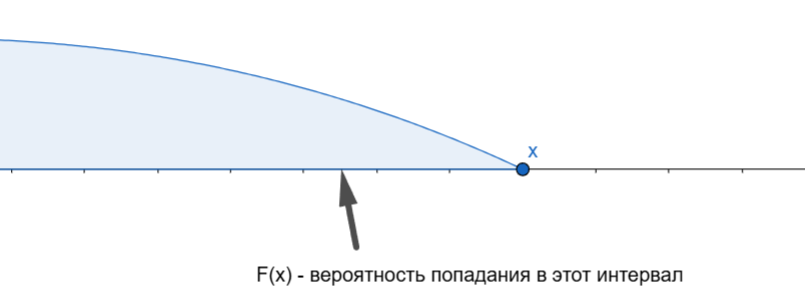
\includegraphics[height=4cm]{probtheory/images/probtheory_2024_10_22_2}

    \begin{minipage}{\textwidth}
        \begin{wrapfigure}{r}{0pt}
            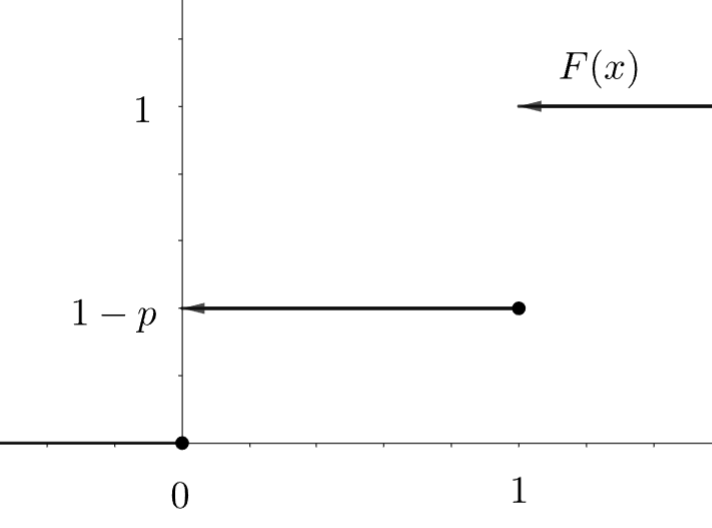
\includegraphics[height=4.5cm]{probtheory/images/probtheory_2024_10_22_3}
        \end{wrapfigure}

        \Ex $\xi \in B_p$ \qquad \begin{tabular}{c|c|c}
            $\xi$ & 0 & 1 \\ \hline
            $p$ & $1 - p$ & $p$ \\
        \end{tabular}
        
        $F_\xi(x) = \begin{cases}0 \quad x \leq 0, \\ 1 - p \quad 0 < x \leq 1, \\ 1 \quad x > 1\end{cases}$

    \end{minipage}

    \subsubsection{Свойства функции распределения}

    1) $F(x)$ ограничена $0 \leq F(x) \leq 1$

    2) $F(x)$ неубывающая функция: $x_1 < x_2 \Longrightarrow F(x_1) \leq F(x_2)$ 

    \begin{MyProof}
        $x_1 < x_2 \Longrightarrow \{\xi < x_1\} \subset \{\xi < x_2\} \Longrightarrow p(\xi < x_1) \leq p(\xi < x_2)$, то есть $F(x_1) \leq F(x_2)$
    \end{MyProof}

    3) $p(\alpha \leq \xi < \beta) = F(\beta) - F(\alpha)$

    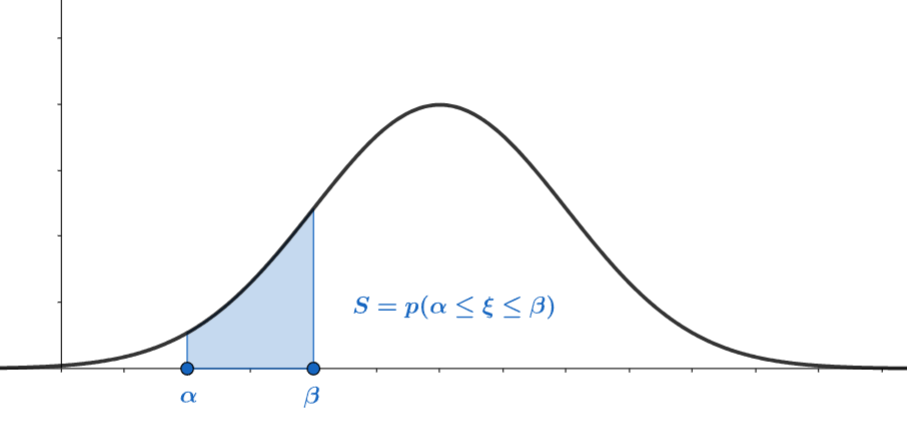
\includegraphics[height=6cm]{probtheory/images/probtheory_2024_10_22_4}

    \begin{MyProof}
        $p(\xi < \beta) = p(\xi < \alpha) + p(\alpha \leq \xi < \beta) \Longrightarrow F(\beta) = F(\alpha) + p(\alpha \leq \xi < \beta)$
    \end{MyProof}
    
    \Notas Функция распределения $F(x)$ - вероятность попадания в интервал $(-\infty; x)$. Так как Борелевская $\sigma$-алгебра порождается такими интервалами,
    то распределение полностью задается этой функцией

    4) $\lim_{x \to -\infty} F(x) = 0; \quad \lim_{x \to +\infty} F(x) = 1$

    \begin{MyProof}
        Так как $F(x)$ монотонна и ограничена, то эти пределы существуют. Поэтому достаточно доказать эти пределы для некоторой последовательности $x_n \to \pm \infty$

        $\letsymbol A_n = \{n - 1 \leq \xi < n, n \in v\}$ - несовместные события, так как $\Real = \bigunion_{n = -\infty}^\infty A_n$, то
        по аксиоме счетной аддитивности, вероятность $p(\xi \in \Real) = 1 = \sum_{n = -\infty}^\infty P(A_n) = \lim_{N \to \infty} \sum_{n = -N}^N p(n - 1 \leq \xi < n) = 
        \lim_{N \to \infty} \sum_{n = -N}^N (F(n) - F(n - 1)) = \lim_{N \to \infty} (F(N) - F(-N - 1)) = \lim_{N \to \infty} F(N) - \lim_{N \to -\infty} F(N) = 1$

        $\Longrightarrow \lim_{N \to \infty} F(N) = 1 + \lim_{N \to -\infty} F(N) $

        Так как $\lim_{N \to \infty} F(N) \leq 1$ и $\lim_{N \to -\infty} F(N) \geq 0$, то $\lim_{N \to \infty} F(N) = 1$ и $\lim_{N \to -\infty} = 0$
    \end{MyProof}
    
    5) $F(x)$ непрерывна слева: $F(x_0 - 0) = F(x_0)$

    \begin{MyProof}
        Этот предел существует в силу монотонности и ограниченности функции, поэтому рассмотрим последовательность событий $B_n = \{x_0 - \frac{1}{n} \leq \xi < x_0, n \in \mathrm{Z}\}$

        Так как $B_1 \supset B_2 \supset \dots \supset B_n \supset \dots$ и $\bigcap_{n = 1}^\infty B_n = \emptyset$

        То по аксиоме непрерывности $p(B_n) \to 0$

        $P(B_n) = F(x_0) - F(x_0 - \frac{1}{n}) \rightarrow 0$

        $F(x_0 - \frac{1}{n}) \to F(x_0)$

        $\lim_{x \to x_0 - 0} F(x) = F(x_0)$
    \end{MyProof}
    
    6) Скачок в точке $x_0$ равен вероятности попадания в данную точку: $F(x_0 + 0) - F(x_0) = p(\xi = x_0)$ или $F(x_0 + 0) = p(\xi = x_0) + p(\xi < x_0) = p(\xi \leq x_0)$

    
    \begin{MyProof}
        Этот предел существует в силу монотонности и ограниченности функции, поэтому рассмотрим последовательность событий $C_n = \{x_0 \leq \xi < x_0 + \frac{1}{n}, n \in \mathrm{Z}\}$

        Так как $C_1 \supset C_2 \supset \dots \supset C_n \supset \dots$ и $\bigcap_{n = 1}^\infty C_n = \emptyset$

        То по аксиоме непрерывности $p(C_n) \to 0$

        $P(C_n) = F(x_0 + \frac{1}{n}) - F(x_0) \rightarrow 0$

        $p(x_0 \leq \xi < x_0 + \frac{1}{n}) + p(\xi = x_0) \rightarrow p(\xi = x_0)$

        $F(x_0 + \frac{1}{n}) - F(x_0) \to p(\xi = x_0)$

        $F(x_0 + 0) - F(x_0) \to p(\xi = x_0)$
    \end{MyProof}
    
    7) Если функция распределения непрерывна в точке $x = x_0$, то очевидно, что вероятность попадания в эту точка $p(\xi = x_0) = 0$ (следствие из 6 пункта)
    
    8) Если $F(x)$ непрерывна $\forall x \in \Real$, то $p(\alpha \leq \xi < \beta) = p(\alpha < \xi < \beta) = p(\alpha \leq \xi \leq \beta) = p(\alpha < \xi \leq \beta) = F(\beta) - F(\alpha)$
    
    \begin{MyTheorem}
        \Ths Случайная величина $\xi$ имеет дискретное распределение тогда и только тогда, когда ее функция распределения имеет ступенчатый вид
    \end{MyTheorem}

    \subsection{Абсолютно непрерывное распределение}

    \Def Случайная величина $\xi$ имеет абсолютно непрерывное распределение, если существует $f_\xi(x)$ такая, что $\forall B \in \mathcal{B}(\Real)
    \ p(\xi \in B) = \int_B f_\xi(x)dx$

    Функция $f_\xi$ называется плотностью распределения случайной величины

    (в определении использует интеграл Лебега, так как $B$ может быть не просто интервалом на $\Real$)

    \subsubsection{Свойства плотности и функции распределения абсолютно непрерывного распределения}

    1) Вероятносто-геометрический смысл плотности: $p(\alpha \leq \xi < \beta) = \int_{\alpha}^\beta f_\xi(x) dx$

    2) Условие нормировки: $\int_{-\infty}^{+\infty} f_\xi(x)dx = 1$

    \begin{MyProof}
        Из определения, если $B = \Real$
    \end{MyProof}

    3) $F_\xi(x) = \int_B f_\xi(x)dx$

    \begin{MyProof}
        Если $B = (-\infty; x)$, то $F_\xi(x) = p(\xi \in (-\infty; x)) = \int_{-\infty}^x f_\xi(x)dx$
    \end{MyProof}

    4) $F_\xi(x)$ непрерывна 
    
    \begin{MyProof}
        Из свойства непрерывности интеграла с верхним переменным пределом
    \end{MyProof}

    5) $F_\xi(x)$ дифференцируема почти везде и $f_\xi(x) = F^\prime_\xi(x)$ для почти всех $x$
    
    \begin{MyProof}
        По теореме Барроу
    \end{MyProof}

    6) $f_\xi(x) \geq 0$ по определению и как производная неубывающей $F_\xi(x)$

    7) $p(\xi = x) = 0 \ \forall x \in \Real$ - так как $F_\xi(x)$ непрерывна

    8) $p(\alpha \leq \xi < \beta) = p(\alpha < \xi < \beta) = p(\alpha \leq \xi \leq \beta) = p(\alpha < \xi \leq \beta) = F(\beta) - F(\alpha)$

    9) \Ths Если $f(x) \leq 0$ и $\int_{-\infty}^{\infty} f(x)dx$ (выполнены свойства 2 и 6), то $f(x)$ - плотность некоторого распределения

    \subsubsection{Числовые характеристики}

    \Def Математическим ожиданием $E\xi$ случайной абсолютно непрерывной величины $\xi$ называется величина $E\xi = \int_{-\infty}^{\infty} xf_\xi(x) dx$ 
    при условии, что данный интеграл сходится абсолютно, то есть $\int_{-\infty}^\infty |x|f_\xi(x)dx < \infty$

    \Def Дисперсией $D\xi$ случайной величины $\xi$ называется величина $D\xi = E(\xi - E\xi)^2 = \int_{-\infty}^\infty (x - E\xi)^2 f_\xi(x) dx$ при условии,
    что данный интеграл сходится

    \Notas Вычислять удобно по формуле $D\xi = E\xi^2 - (E\xi)^2 = \int_{-\infty}^\infty x^2 f_\xi(x)dx - (E\xi)^2$

    \Def Среднее квадратическое отклонение $\sigma_\xi = \sqrt{D\xi}$ определяется, как корень дисперсии

    Смысл этих величин такой же, как и при дискретном распределении. Также свойства аналогичны тем, что и при дискретном распределении

    \subsubsection{Другие числовые характеристики}

    $m_k = E\xi^k = \int_{-\infty}^\infty x^k f_\xi(x)dx$ - момент $k$-ого порядка

    $\mu_k = E(\xi - E\xi)^k = \int_{-\infty}^\infty (x - E\xi)^k f_\xi(x)dx$ - центральный момент $k$-ого порядка

    \Def Медианой $Me$ абсолютно непрерывной случайной величины $\xi$ называется значение случайной величины $\xi$, такое что $p(\xi < Me) = p(\xi > Me) = \frac{1}{2}$
    
    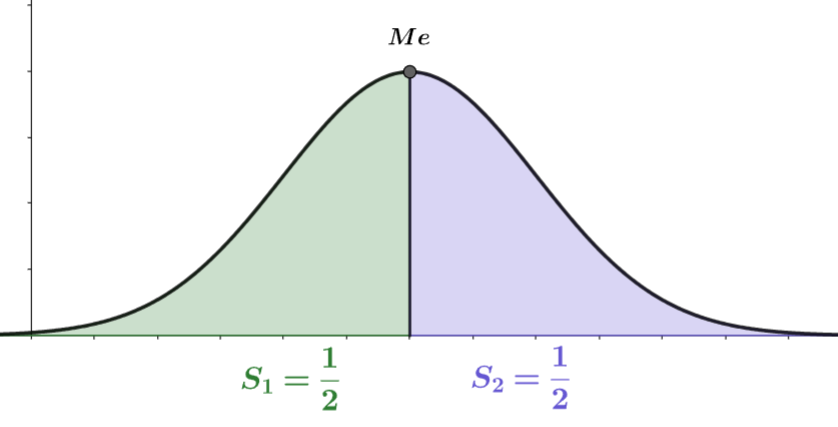
\includegraphics[height=4cm]{probtheory/images/probtheory_2024_10_22_5}

    \Def Модой $Mo$ случайной величины $\xi$ называется точка локального максимума плотности

    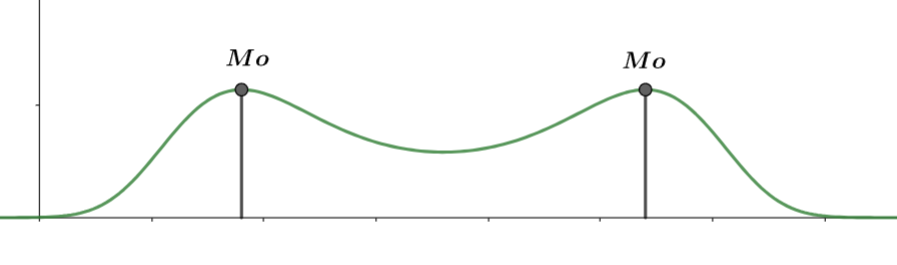
\includegraphics[height=4cm]{probtheory/images/probtheory_2024_10_22_6}

    \subsection{Сингулярное распределение}

    \Def Случайная величина $\xi$ имеет случайное распределение, если $\exists B$ - Борелевское множество с нулевой мерой Лебега $\lambda(B) = 0$, такое что $p(\xi \in B) \in 1$, но $P(\xi = x) = 0 \ \, \forall x \in B$

    \Nota Такое Борелевское множество состоит из несчетного множества точек, так как в протичном случае по аксиоме счетной аддитивности $p(\xi \in B) = 0$. То есть 
    при сингулярном распределении случайная величина $\xi$ распределена на несчетном множестве меры 0

    \Notas Так как $p(\xi = x) = 0 \  \forall x$, $F_\xi$ непрерывна.

    \smallvspace
    
    \begin{minipage}{\textwidth}
        \begin{wrapfigure}{r}{0pt}
            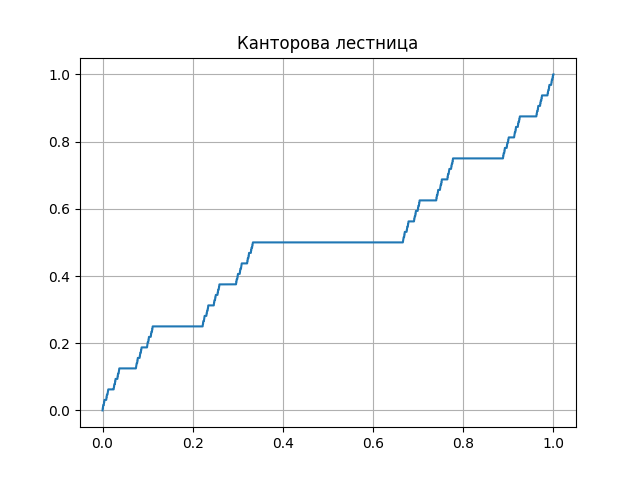
\includegraphics[width=7cm]{probtheory/images/probtheory_2024_10_22_1}
        \end{wrapfigure}

        % import matplotlib.pyplot as plt
        % import numpy

        % cache = {}

        % def f(x, c=0):
        %     if c >= 100:
        %         return x

        %     if x not in cache:
        %         cache[x] = 0 if x <= 0 else \
        %             1/2 * f(3 * x, c+1) if x <= 1/3 else \
        %             1/2 if x <= 2/3 else \
        %             1/2 + 1/2 * f(3 * x - 2, c+1) if x <= 1 else \
        %             1 

        %     return cache[x]

        % x_domain = numpy.arange(0, 1.001, 0.0001)
        % plt.plot(x_domain, [f(i) for i in x_domain])
        % plt.title("Канторова лестница")
        % plt.grid(True)
        % plt.show()

        \Exs Сингулярное распределение получим, если возьмем случайную величину, функция распределения которой - 
        лестница Кантора
    
        $F_\xi(x) = \begin{cases}0 \quad x \leq 0, \\ \frac{1}{2}F(3x) \quad 0 < x \leq \frac{1}{3}, \\ \frac{1}{2} \quad \frac{1}{3} < x \leq \frac{2}{3}, \\ \frac{1}{2} + \frac{1}{2}F(3x - 2) \quad \frac{2}{3} < x \leq 1, \\ 1 \quad x > 1\end{cases}$
    \end{minipage}

    \begin{MyTheorem}
        \ThNs{Лебега}

        $\letsymbol F_\xi(x)$ - функция распределения $\xi$. Тогда $F_\xi(x) = p_1 F_1(x) + p_2 F_2(x) + p_3 F_3(x)$, где $p_1 + p_2 + p_3 = 1$

        $F_1$ - функция дискретного распределения

        $F_2$ - функция абсолютно непрерывного распределения

        $F_3$ - функция сингулярного распределения

        То есть существуют только дискретное, абсолютно непрерывное, сингулярное распределения и их смеси
    \end{MyTheorem}
% end probtheory_2024_10_22.tex

% begin probtheory_2024_10_29.tex

    \section{Лекция 9}

    \subsection{Стандартное абсолютно непрерывное распределение}

    \subsubsection{I. Равномерное распределение}

    \Defs Случайная величина $\xi$ имеет равномерное распределение $\xi \in u(a, b)$, если ее плотность
    на этом отрезке постоянна

    Получаем функцию плотности $f_\xi(x) = \begin{cases}0, \quad x < a \\ \frac{1}{b - a}, \quad a \leq x < b \\ 0 \quad x \geq b\end{cases}$ \hfill {\scriptsize $\frac{1}{b - a}$ из усл. нормировки}

    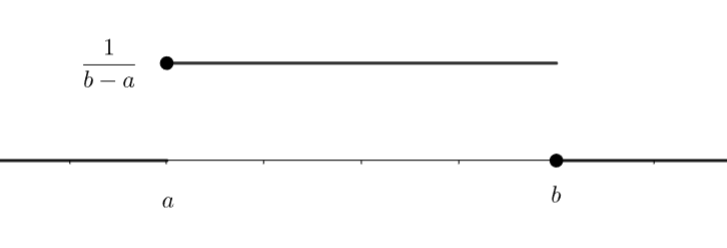
\includegraphics[height=4cm]{probtheory/images/probtheory_2024_10_29_1}

    Из этого функция распределения $F(x) = \int_{-\infty}^\infty f(x)dx = \begin{cases}0, \quad x < a \\ \frac{x - a}{b - a}, \quad a \leq x < b \\ 1 \quad x \geq b\end{cases}$

    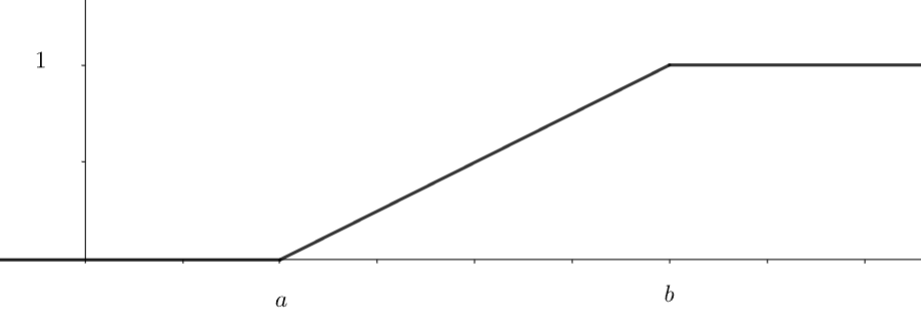
\includegraphics[height=4cm]{probtheory/images/probtheory_2024_10_29_2}

    \textbf{Числовые характеристики}:

    $E\xi = \int_{-\infty}^\infty x f(x) dx = \int_a^b x \frac{1}{b - a} dx = \frac{1}{b - a} \frac{x^2}{2} \Big|_a^b = \frac{b^2 - a^2}{2(b - a)} = \frac{a + b}{2}$

    $E\xi^2 = \int_{-\infty}^\infty x^2 f(x) dx = \int_a^b x^2 \frac{1}{b - a} dx = \frac{1}{b - a} \frac{x^3}{3} \Big|_a^b = \frac{b^3 - a^3}{3(b - a)} = \frac{b^2 + ab + a^2}{3}$

    $D\xi = E\xi^2 - (E\xi)^2 = \frac{b^2 + ab + a^2}{3} - \left(\frac{a + b}{2}\right)^2 = \frac{b^2 - 2ab + a^2}{12} = \frac{(b - a)^2}{12}$
    
    $\sigma = \sqrt{D\xi} = \frac{b - a}{2\sqrt{3}}$

    $p(\alpha < \xi < \beta) = \frac{\beta - \alpha}{b - a}$ при условии, что $\alpha, \beta \in [a, b]$

    \Nota Примеры равномерного распределения: задача со временем, датчики случайных чисел имеют стандартное равномерное распределение $u(0, 1)$

    \subsubsection{II. Показательное распределение}

    \Defs Случайная величина $\xi$ имеет показательное (или экспоненциальное) распределение с параметром $\alpha > 0$ (обозн. $\xi \in E_\alpha$),
    если ее плотность имеет вид:

    \[f_\xi(x) = \begin{cases}0, \quad x < 0 \\ \alpha e^{-\alpha x}, \quad x \geq 0\end{cases}\]

    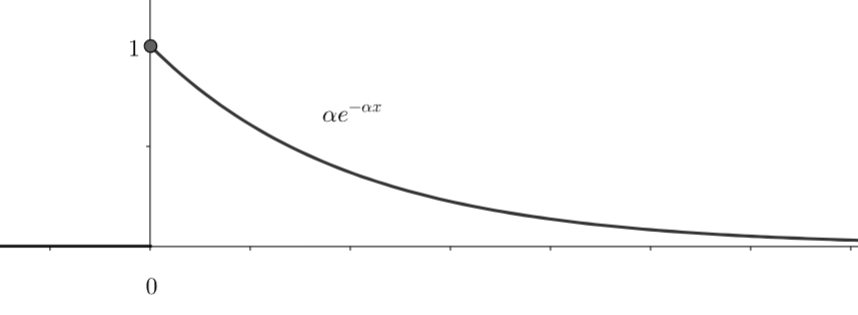
\includegraphics[height=4cm]{probtheory/images/probtheory_2024_10_29_3}

    Функция распределения $F_\xi(x) = \begin{cases}0, \quad x < 0 \\ \int_0^x \alpha e^{-\alpha x} = 1 - e^{-\alpha x}, \quad x \geq 0\end{cases}$

    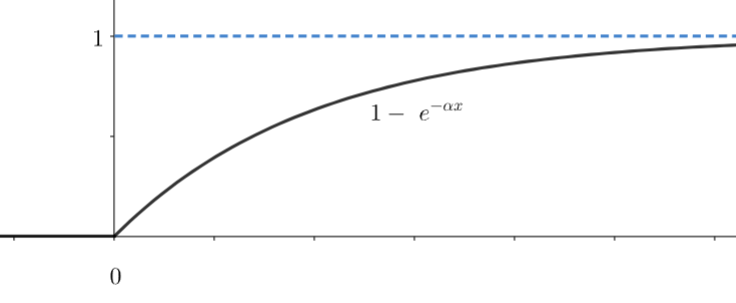
\includegraphics[height=4cm]{probtheory/images/probtheory_2024_10_29_4}

    \textbf{Числовые характеристики}:

    $E\xi = \int_{-\infty}^\infty x f(x) dx = \int_0^\infty x \alpha e^{-\alpha x} dx = \left[\begin{matrix}u = x & du = dx \\ dv = \alpha e^{-\alpha x} \alpha x & v = -e^{-\alpha x}\end{matrix}\right] = -xe^{-\alpha x} \Big|_0^\infty + \int_0^\infty e^{-\alpha x} dx = 
    -\lim_{x \to \infty} \frac{x}{e^{\alpha x}} - \frac{1}{\alpha} e^{-\alpha x} \Big|_0^\infty = -\lim_{x \to \infty} \frac{1}{\alpha e^{\alpha x}} - \frac{1}{\alpha} (\lim_{x \to \infty} e^{-\alpha x} - 1) = \frac{1}{\alpha}$


    $E\xi^2 = \int_{-\infty}^\infty x^2 f(x) dx = \int_0^\infty x^2 \alpha e^{-\alpha x} dx = \left[\begin{matrix}u = x^2 & du = 2xdx \\ dv = \alpha e^{-\alpha x} \alpha x & v = -e^{-\alpha x}\end{matrix}\right] = -x^2 e^{-\alpha x} \Big|_0^\infty + 2\int_0^\infty x e^{-\alpha x} dx = 
    \frac{2}{\alpha} \int_0^\infty \alpha x e^{-\alpha x} = \frac{2}{\alpha} E\xi = \frac{2}{\alpha^2}$

    $D\xi = E\xi^2 - (E\xi)^2 = \frac{2}{\alpha^2} - \left(\frac{1}{\alpha}\right)^2 = \frac{1}{\alpha^2}$
    
    $\sigma = \sqrt{D\xi} = \frac{1}{\alpha}$

    $p(\alpha < \xi < \beta) = F(b) - F(a) = e^{-a\alpha} - e^{-b\alpha} \quad\quad\quad a, b \geq 0$

    \Nota Из непрерывных случайных величин только показательная обладает свойством нестарения

    \begin{MyTheorem}
        \Ths $\letsymbol \xi \in E_\alpha$. Тогда $p(\xi < x + y \ | \ \xi > x) = p(\xi > y) \quad\quad \forall x, y > 0$
    \end{MyTheorem}

    \begin{MyProof}
        $\Box$

        $p(\xi < x + y \ | \ \xi > x) = p(\xi > y) = \frac{p(\xi > x + y, \xi > x)}{p(\xi > x)} = \frac{1 - p(\xi < x + y)}{1 - p(\xi < x)} = 
        \frac{1 - F(x + y)}{1 - F(x)} = \frac{e^{-\alpha(x + y)}}{e^{-\alpha x}} = e^{-\alpha y} = 1 - (1 - e^{-\alpha y}) = 1 - p(\xi < y) = p(\xi > y)$

        $\Box$
    \end{MyProof}

    \ExNs{1} Время работы надежной микросхемы до поломки

    \ExNs{2} Время между появлениями двух редких событий (через схему Пуассона)

    \Notas Применется в системах массового обслуживания, теория надежности


    \subsubsection{III. Нормальное распределение (Гауссовское)}

    \Def Случайная величина $\xi$ имеет нормальное распределение с параметрами $a$ и $\sigma^2$ (обозн. $\xi \in N(a, \sigma^2)$), если
    ее плотность имеет вид:

    \[f(x) = \frac{1}{\sigma \sqrt{2\pi}} e^{-\frac{(x - a)^2}{2\sigma^2}}, \quad -\infty < x < \infty\]

    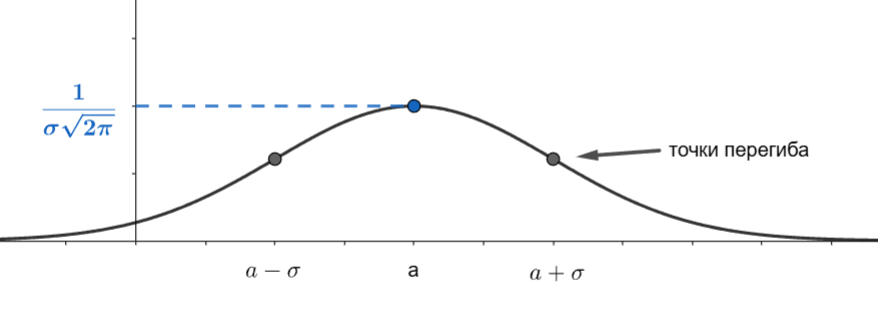
\includegraphics[height=4cm]{probtheory/images/probtheory_2024_10_29_5}

    Смысл параметров распределения: $a = E\xi$ - матожидание и медиана, $\sigma$ - СКО, а $D\xi = \sigma^2$

    Функция распределения: $F(x) = \frac{1}{\sigma \sqrt{2\pi}} \int_{-\infty}^x e^{-\frac{(t - a)^2}{2\sigma^2}} dt$

    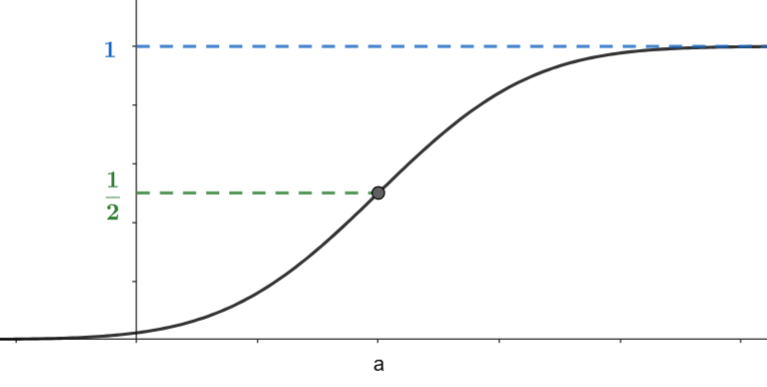
\includegraphics[height=4cm]{probtheory/images/probtheory_2024_10_29_6}

    Проверим корректность определения - условие нормировки. Покажем, что $\int_{-\infty}^\infty f(x)dx = 1$

    $\int_{-\infty}^\infty \frac{1}{\sigma \sqrt{2\pi}} e^{-\frac{(x - a)^2}{2\sigma^2}} dx = \left[\begin{matrix}t = \frac{x - a}{\sigma \sqrt{2}} & dt = \frac{dx}{\sigma\sqrt{2}} \\ t (\pm \infty) = \pm \infty & dx = \sigma\sqrt{2}dt\end{matrix}\right] = 
    \int_{-\infty}^\infty \frac{1}{\sigma\sqrt{2\pi}} e^{-t^2} \sigma\sqrt{2} dt = \frac{1}{\sqrt{\pi}} \int_{-\infty}^{\infty} e^{-t^2} dt = \frac{1}{\sqrt{\pi}} \sqrt{\pi} = 1$ - верно

    Ясно, что $m_k = \int_{-\infty}^\infty x^k f(x) dx = \int_{-\infty}^\infty x^k \frac{1}{\sigma \sqrt{2\pi}} e^{-\frac{(x - a)^2}{2\sigma^2}} dx$ - интеграл сходится абсолютно для любого $k$ (степень $e$ задавит полином)

    $E\xi = m_1 = \int_{-\infty}^\infty x^k \frac{1}{\sigma \sqrt{2\pi}} e^{-\frac{(x - a)^2}{2\sigma^2}} dx = a$ в силу симметрии

    Найдем дисперсию при помощи дифференцирования интеграла по параметру: 
    
    Из условия нормировки $\int_{-\infty}^\infty \frac{1}{\sigma \sqrt{2\pi}} e^{-\frac{(x - a)^2}{2\sigma^2}} dx = 1$

    $\frac{1}{\sqrt{2\pi}} \int_{-\infty}^\infty e^{-\frac{(x - a)^2}{2\sigma^2}} dx = \sigma$
    
    $\frac{1}{\sqrt{2\pi}} \int_{\infty}^\infty e^{-\frac{(x - a)^2}{2\sigma^2}} \left(-\frac{(x - a)^2}{2} (-\sigma^{-3})\right) dx = 1$
    
    $\frac{1}{\sigma\sqrt{2\pi}} \int_{\infty}^\infty (x - a)^2 e^{-\frac{(x - a)^2}{2\sigma^2}} dx = \sigma^2 = D\xi$, получаем, что $\sigma$ - СКО

    \mediumvspace

    \textbf{Стандартное нормальное распределение}

    \Def Стандартным нормальным распределением называется нормальное распределение с параметрами $a = 0, \sigma^2 = 1$: $\xi \in N(0, 1)$

    Плотность: $\phi(x) = \frac{1}{\sqrt{2\pi}} e^{-\frac{x^2}{2}}$ - функция Гаусса

    $E\xi = 0; \ D\xi = 1$

    Распределение: $F_0(x) = \frac{1}{\sqrt{2\pi}} \int_{-\infty}^x e^{-\frac{z^2}{2}} dz$ - функция стандартного нормального распределения

    Заметим, что $F_0(x) = \frac{1}{\sqrt{2\pi}} \int_{-\infty}^0 e^{-\frac{z^2}{2}} dz + \frac{1}{\sqrt{2\pi}} \int_0^x e^{-\frac{z^2}{2}} dz = \frac{1}{2} + \Phi(x)$, где $\Phi(x)$ - функция Лапласа

    Функция Лапласа нечетная и из соображения симметрии легко вычисляется для отрицательных $x$, однако большинство ПО используют $F_0(x)$
    
    \subsubsection{Связь между нормальным и стандартным нормальным распределениями}

    1) $\letsymbol \xi \in N(a, \sigma^2)$. Тогда $F_\xi(x) = F_0\left(\frac{x - a}{\sigma}\right)$

    \begin{MyProof}
        $\Box$
        
        $F_\xi(x) = \frac{1}{\sigma\sqrt{2\pi}} \int_{-\infty}^x e^{-\frac{(t - a)^2}{2\sigma^2}} dt = \left[\begin{matrix}z = \frac{t - a}{\sigma} & t = \sigma z + a & dt = \sigma dz \\ z (-\infty) = -\infty & z(x) = \frac{x - a}{\sigma} & \end{matrix}\right] = 
        \frac{1}{\sigma\sqrt{2\pi}} \int_{-\infty}^\frac{x - a}{\sigma} e^{-\frac{z^2}{2}} \sigma dz = \frac{1}{\sqrt{2\pi}} \int_{-\infty}^\frac{x - a}{\sigma} e^{-\frac{z^2}{2}} dz = F_0\left(\frac{x - a}{\sigma}\right)$
        
        $\Box$
    \end{MyProof}

    2) Если $\xi \in N(a, \sigma^2)$, то $\eta = \frac{\xi - a}{\sigma} \in N(0, 1)$ (процесс $\xi \to \eta$ называется стандартизацией)

    \begin{MyProof}
        $\Box$
        
        $F_\eta(x) = p(\eta < x) = p\left(\frac{\xi - a}{\sigma} < x\right) = p(\xi < \sigma x + a) = F_\xi(\sigma x + a) = F_0\left(\frac{\sigma x + a - a}{\sigma}\right) = F_0(x)$, так как $F_\eta(x) = F_0(x)$, то $\eta \in N(0, 1)$
        
        $\Box$
    \end{MyProof}

    3) $\letsymbol \xi \in N(a, \sigma^2)$. Тогда $p(\alpha < \xi < \beta) = \Phi\left(\frac{\beta - a}{\sigma}\right) - \Phi\left(\frac{\alpha - a}{\sigma}\right)$

    \begin{MyProof}
        $p(\alpha < \xi < \beta) = F_\xi(\beta) - F_\xi(\alpha) = F_0\left(\frac{\beta - a}{\sigma}\right) - F_0\left(\frac{\alpha - a}{\sigma}\right) = \Phi\left(\frac{\beta - a}{\sigma}\right) - \Phi\left(\frac{\alpha - a}{\sigma}\right)$
    \end{MyProof}

    4) Вероятность попадания в симметричный интервал (вероятность отклонения случайной величины от матожидания) 
    $p(|\xi - a| < t) = 2\Phi\left(\frac{t}{\sigma}\right)$

    \begin{MyProof}
        $p(|\xi - a| < t) = p(-t < \xi - a < t) = p(a - t < \xi < a + t) = \Phi\left(\frac{a + t - a}{\sigma}\right) - \Phi\left(\frac{a - t - a}{\sigma}\right) = \Phi\left(\frac{t}{\sigma}\right) - \Phi\left(-\frac{t}{\sigma}\right) = 2\Phi\left(\frac{t}{\sigma}\right)$
    \end{MyProof}

    \Notas Если через $F_0(x)$, то $p(|\xi - a| < t) = 2\F_0\left(\frac{t}{\sigma}\right) - 1$

    5) Правило 3 \enquote{сигм}: $p(|\xi - a| < 3\sigma) \approx 0.9973$ - попадание случайной величины нормального распределения в интервал $(a - 3\sigma, a + 3\sigma)$ близко к 1

    \begin{MyProof}
        $p(|\xi - a| < 3\sigma) = 2\Phi\left(\frac{3\sigma}{\sigma}\right) = 2\Phi(3) = 2 \cdot 0.49685 = 0.9973$
    \end{MyProof}

    6) Свойство линейности: если случайная величина $\xi \in N(a, \sigma^2)$, то $\eta = \gamma \xi + b \in N(a \gamma + b, \gamma^2 \sigma^2)$ (можем доказать при помощи свойств ранее, но мы докажем позже, используя другие методы)

    7) Устойчивость относительно суммирования: если случайные величины $\xi_1 \in N(a_1, \sigma_1^2), \xi_2 \in N(a_2, \sigma_2^2)$, и они независимы, то $\xi_1 + \xi_2 \in N(a_1 + a_2, \sigma^2_1 + \sigma^2_2)$

    \subsubsection{Коэффициенты асимметрии и эксцесса}

    \DefN{1} Асимметрией распределения называется число $A_s = E\left(\frac{\xi - a}{\sigma}\right)^3 = \frac{\mu^3}{\sigma^3}$

    \DefNs{2} Эксцессом распределения называется число $E_s = E\left(\frac{\xi - a}{\sigma}\right)^4 - 3 = \frac{\mu^4}{\sigma^4} - 3$

    \Notas Если случайная величина $\xi \in N(a, \sigma^2)$, то $A_s = E_s = 0$, таким образом, отличие этих характеристик от нуля характеризирует 
    степень отклонения распределения. Благодаря этим и другим параметрам, можно проверять на практике, является ли распределение нормальным 
% end probtheory_2024_10_29.tex

% begin probtheory_2024_11_05.tex

    \section{Лекция 10}

    \subsection{Преобразование случайных величин}

    \subsubsection{Стандартизация случайной величины}

    \Def Пусть имеется случайная величина $\xi$. Соответствующей ей стандартной величиной называется
    случайная величина $\eta = \frac{\xi - E\xi}{\sigma}$

    \textbf{Свойства}:

    $E\eta = 0; D\eta = 1$

    \begin{MyProof}
        $E\eta = E \frac{\xi - E\xi}{\sigma} = \frac{1}{\sigma} (E\xi - E\xi) = 0$

        $D\eta = D \frac{\xi - E\xi}{\sigma} = \frac{1}{\sigma^2} D\xi = 1$
    \end{MyProof}

    Стандартизованная случайная величина не имеет единиц измерения, таким образом, ее свойства от них не зависят

    \mediumvspace

    \underline{Задача}: пусть имеется функция $g(x)$ и случайная величина $\xi$, $\eta = g(\xi)$. Определить ее характеристики

    \Nota Если $\xi$ - дискретная случайная величина, то ее законы распределения находятся просто: значения $x_i$ в верхней строке заменяем $g(x_i)$, вероятности остаются прежние.
    Поэтому будем рассматривать непрерывной случайной величины $\xi$

    \Notas Возможна ситуация, когда $\xi$ - абсолютно непрерывная случайная величина, $g(x)$ - непрерывна, но $g(\xi)$ имеет дискретное распределение

    \subsubsection{Линейное преобразование}

    \begin{MyTheorem}
        \Ths Пусть $\xi$ имеет плотность $f_\xi(x)$, тогда $\eta = a\xi + b$, где $a \neq 0$, имеет плотность $f_\eta(x) = \frac{1}{|a|}f_\xi(\frac{f - b}{a})$
    \end{MyTheorem}

    \begin{MyProof}
        Пусть $a > 0$, тогда $F_\eta(x) = p(\eta < x) = p(a\xi + b < x) = p(\xi < \frac{x - b}{a}) = \int_{-\infty}^{\frac{x - b}{a}} f_\xi(t) dt = 
        \left[\begin{matrix}t = \frac{y - b}{a} & dt = \frac{1}{a} dy & y = at + b \\ y(-\infty) = -\infty & y(\frac{x - b}{a}) = x\end{matrix}\right] = 
        \int_{-\infty}^x \frac{1}{a} f_\xi(\frac{y - b}{a}) dy \Longrightarrow \eta = \frac{1}{|a|} f_\xi (\frac{x - b}{a})$

        Пусть $a < 0$, тогда $F_\eta(x) = p(\eta < x) = p(a\xi + b < x) = p(\xi > \frac{x - b}{a}) = \int_{\frac{x - b}{a}}^{\infty} f_\xi(t) dt = 
        \left[\begin{matrix}t = \frac{y - b}{a} & dt = \frac{1}{a} dy & y = at + b \\ y(\infty) = -\infty & y(\frac{x - b}{a}) = x\end{matrix}\right] = 
        -\int_{-\infty}^x \frac{1}{a} f_\xi(\frac{y - b}{a}) dy \Longrightarrow \eta = \frac{1}{|a|} f_\xi (\frac{x - b}{a})$
    \end{MyProof}

    \underline{Следствие}

    1) Если $\xi \in N(a, \sigma^2)$, то $\eta = \gamma \xi + b \in N(a\gamma + b; \gamma^2 \sigma^2)$

    \begin{MyProof}
        Так как $\xi \in N(a, \sigma^2)$, то $f_\xi(x) = \frac{1}{\sigma\sqrt{2\pi}} e^{-\frac{(x - a)}{2\sigma^2}}, x \in \Real$

        Тогда $f_\eta(x) = \frac{1}{|\gamma|} \cdot \frac{1}{\sigma\sqrt{2\pi}} e^{-\frac{(\frac{x - b}{\gamma} - a)^2}{2\sigma^2}} = \frac{1}{|\gamma|\sigma\sqrt{2\pi}} e^{-\frac{(x - b - a\gamma)^2}{2\sigma^2\gamma^2}} \Longrightarrow \eta \in N(b + a\gamma; \sigma^2\gamma^2)$
    \end{MyProof}

    2) Если $\eta \in N(0, 1)$ - стандартное нормальное распределение, то $\xi = \sigma \eta + a \in N(a, \sigma^2)$

    3) Если $\eta \in U(0, 1)$ - стандартное равномерное распределение и $a > 0$, то $\xi = a\eta + b \in U(b, a + b)$

    4) Если $\xi \in E_\alpha$, то $\alpha \xi \in E_1$

    \subsubsection{Монотонное преобразование}

    \begin{MyTheorem}
        \Ths Пусть $f_\xi(x)$ - плотность случайной величины $\xi$, $g(x)$ - строго монотонная функция. Тогда 
        случайная величина $\eta = g(\xi)$ имеет плотность

        \[f_\eta(x) = |h^\prime(x)| f_\xi(h(x)), \qquad\qquad \text{где } h(g(x)) = x\]
    \end{MyTheorem}

    Если $g(x)$ не является монотонное функцией, то поступаем следующим образом: разбиваем $g(x)$ на интервалы монотонности, 
    для каждого $i$-ого интервала находимся $h_i(x)$ и плотность случайной величины ищем по \textit{формуле Смирнова}: 
    $f_\eta(x) = \sum_{i = 0}^n |h_i^\prime(x)| f_\xi(h_i(x))$
    
    \subsubsection{Квантильное преобразование}

    \begin{MyTheorem}
        \ThNs{1} Пусть функция распределения случайной величины $\xi$ $F_\xi(x)$ - непрерывная функция. 
        Тогда $\eta = F(\xi) \in U(0, 1)$ - стандартное равномерное распределение
    \end{MyTheorem}

    \begin{MyProof}
        Ясно, что $0 \leq \eta \leq 1$

        a) $F(x)$ - строго возрастающая функция. Тогда $\exists F^{-1}(x)$ - обратная, $F_\eta(x) = p(\eta < x) = p(F(\xi) < x) = 
        \begin{cases}0, & x < 0 \\ p(\xi < F^{-1}(x)) = F(F^{-1}(x)) = x, & 0 \leq x \leq 1 \text{ - функция распределения } U(0, 1) \\ 1, & x > 1 \end{cases}$

        б) $F(x)$ - не является строго возрастающей функцией - то есть существуют участки постоянства, в этом случае
        определим $F^{-1}$ как $F^{-1}(x) = \min_{t} (t \ | \ F(t) = x)$ - то есть берем самую левую точку такого интервала

        Тогда снова будет при $0 \leq x \leq 1 \ F_\eta(x) = p(\eta < x) = p(F(\xi) < x) = F(F^{-1}(x)) = x$

    \end{MyProof}

    Сформулируем обратную теорему: пусть $F(x)$ - функция распределения (необязательно непрерывная) случайной величины $\xi$,
    обозначим $F^{-1}(x) = \inf_t (t \ | F(t) \geq x)$.

    В случае непрерывной $F(x)$ это определение совпадет с предыдущем

    \begin{MyTheorem}
        \ThNs{2} Пусть $\eta \in U(0, 1)$ - стандартное равномерное распределение, $F(x)$ - произвольная функция распределения. 
        Тогда $\xi = F^{-1}(\eta)$ имеет функцию распределения $F(x)$
    \end{MyTheorem}

    Данное преобразование $\xi = F^{-1}(\eta)$ называют квантильным

    Доказательство аналогично предыдущей теореме
    
    Смысл: датчики случайных чисел имеют стандартное равномерное распределение, из теоремы следует, что при помощи
    датчика случайных чисел и квантильного преобразования мы сможем смоделировать любое нужно распределение

    \ExN{1} Смоделируем показательное распределение $E_\alpha: \ F_\alpha(x) = \begin{cases}0, & x < 0 \\ 1 - e^{-\alpha x}, & x \geq 0\end{cases}$

    $\eta = 1 - e^{-\alpha x}, \ e^{-\alpha x} = 1 - \eta, \ x = -\frac{1}{\alpha} \ln(1 - \eta)$ - функция, обратная к $F_\alpha(x)$

    Если $\eta \in U(0, 1)$, то $\xi = -\frac{1}{\alpha} \ln(1 - \eta) \in E_\alpha$

    \ExN{2} $\xi \in N(0, 1), \ F_0(x) = \frac{1}{\sqrt{2\pi}} \int_{-\infty}^x e^{-z^2}{2} dz$

    Пусть $F_0^{-1}(x)$ - функция обратная к $F_0(x)$

    Если $\eta \in U(0, 1)$, то $F_0^{-1}(\eta) \in N(0, 1)$

    \subsection{Характеристики преобразованной случайной величины}

    \begin{MyTheorem}
        \Ths Если $\xi$ - дискретная случайная величина, то $Eg(\xi) = \sum_{i = 1}^\infty g(x_i) \cdot p_i = \sum_{i = 1}^\infty g(x_i) \cdot p(\xi = x_i)$

        Для непрерывной случайной величины $Eg(\xi) = \int_{-\infty}^{\infty} g(x) f_\xi(x) dx$
    \end{MyTheorem}

    \subsubsection{Свойства моментов}

    1) Если $\xi \geq 0$, то $E\xi \geq 0$

    2) Если $\xi \leq \eta$, то $E\xi \leq E\eta$

    \begin{MyProof}
        $\xi \leq \eta \Longrightarrow \eta - \xi \geq 0 \Longrightarrow E(\eta - \xi) \geq 0 \Longrightarrow E\eta - E\xi \geq 0 \Longrightarrow E\eta \geq E\xi$
    \end{MyProof}

    3) Если $|\xi| \leq |\eta|$, то $E|\xi|^k \leq E|\eta|^k$

    4) Если существует момент $m_t$ случайной величины $\xi$, то существует $m_s$ при $s < t$ (при условии, что интеграл/сумма сходятся)

    \begin{MyProof}
        Пусть $s < t$. Тогда $|x|^s \leq \min(1, |x|^t) \leq 1 + |x|^t$, так как при $|x| < 1, \ |x|^s \leq 1$ и при $|x| \geq 1, \ |x|^s \leq |x|^t$
    
        $E|\xi|^s \leq E|\xi|^t + 1$ и если $E|\xi|^t$ существует (конечно), то $\exists E|\xi|^s$
    
    \end{MyProof}

    \begin{MyTheorem}
        \ThNs{Неравенство Йенсена} Пусть функция $g(x)$ выпукла вниз, тогда для любой случайной величины $\xi$

        \[Eg(\xi) \geq g(E\xi)\]
    \end{MyTheorem}

    \Nota Если $g(x)$ выпукла вверх, знак неравенства меняется
    
    \begin{MyProof}
        Если $g(x)$ выпукла вниз, то в любой ее точке, можно провести прямую, лежащую не выше графика функции. То есть для 
        любой $x_0$ существует $k(x_0)$ такой, что $g(x) \geq g(x_0) + k(x_0) (x - x_0)$

        Пусть $x_0 = E\xi$, $g(E\xi) \geq g(E\xi) + k(E\xi) (x - E\xi)$

        $Eg(\xi) \geq Eg(E\xi) + k(E\xi) \underset{= 0}{(E\xi - E\xi)}$

        $Eg(\xi) \geq g(E\xi)$
    \end{MyProof}

    % ниче не понял, maybe wrong

    Следствие:

    $Ee^\xi \geq e^{E\xi}, \quad E\xi^2 \geq (E\xi)^2, \quad E|q| \geq |Eq|, \quad E\ln(\xi) \leq \ln(E\xi), \quad E\frac{1}{\xi} \geq \frac{1}{E\xi}$ при $\xi > 0$


    \begin{minipage}{\textwidth}
        \begin{wrapfigure}{r}{0pt}
            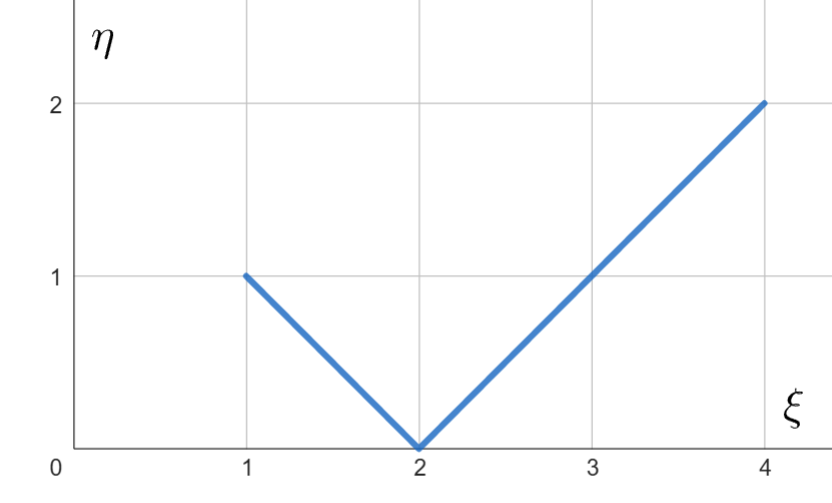
\includegraphics[width=7cm]{probtheory/images/probtheory_2024_11_05_1}
        \end{wrapfigure}

        \Ex на формулу Смирнова: дана плотность распределения
    
        $f_\xi(x) = \begin{cases}0, & x < 1 \\ \frac{4}{3x^2}, & 1 \leq x \leq 4, 0 & x > 4\end{cases}$
    
        Найти $f_\eta$ для $\eta = |\xi - 2|$

        \underline{Решение}

        $\xi \in [1, 4], \quad \eta \in [0, 2]$
    \end{minipage}

    \begin{cases}
        0 \leq \eta \leq 1 \Longrightarrow h_1(\eta) = \eta + 2 \text{ и } h_2(\eta) = 2 - \eta & \text{\qquad - 2 ветви} \\ 
        1 < \eta \leq 2 \Longrightarrow h_1(\eta) = \eta + 2 & \text{\qquad - 1 ветвь}
    \end{cases}

    $h_1^\prime(\eta) = 1, h_2^\prime(\eta) = -1 \qquad |h_1^\prime(\eta)| = |h_2^\prime(\eta)| = 1$

    $f_\eta(x) = \sum_i |h_i^\prime(x)| f_\xi(h_i(x))$

    $f_\eta(x) = \begin{cases}0, & x < 0 \\ \frac{4}{3}\left(\frac{1}{(x + 2)^2} + \frac{1}{(2 - x)^2}\right), & 0 \leq x \leq 1 \\ \frac{4}{3}\frac{1}{(x + 2)^2}, & 1 < x \leq 2 \\ 0 & x > 2\end{cases}$
% end probtheory_2024_11_05.tex

% begin probtheory_2024_11_12.tex

    \section{Лекция 11}

    \subsection{Сходимость случайных величин}

    Рассмотрим 3 вида сходимости:

    \begin{itemize}
        \item Сходимость \enquote{почти наверное}

        \Defs Случайная величина $\xi$ имеет свойство $\mathrm{Cond}$ \enquote{почти наверное}, если вероятность $p(\xi \text{ имеет свойство } \mathrm{Cond}) = 1$
    
        \Nota То есть $p(\xi \text{ не имеет свойство } \mathrm{Cond}) = 0$

        $p(\omega \in \Omega \ | \ \xi(\omega) \text{ не имеет св-во } \mathrm{Cond})$

        \Def Последовательность случайных величин $\{\xi_n\}$ сходится \enquote{почти наверное} к случайной величине $\xi$ при $n \to \infty$ ($\xi_n \overset{\text{п. н.}}{\longrightarrow} \xi$), 
        если $p(\omega \in \Omega \ | \ \xi_n(\omega) \underset{n \to \infty}{\longrightarrow} \xi(\omega)) = 1$

        \item Сходимость по вероятности

        \Defs Последовательность случайных величин $\{\xi_n\}$ сходится по вероятности к случайной величине $\xi$ при $n \to \infty$
        ($\xi_n \overset{p}{\longrightarrow} \xi$), если $\forall \varepsilon > 0 \quad p(|\xi_n - \xi| < \varepsilon) \underset{n \to \infty}{\longrightarrow} 1$
        
        \Nota Не надо думать, что из сходимости по вероятности следует сходимости математического ожидания $\xi_n \overset{p}{\longrightarrow} \xi \centernot{\Longrightarrow} E\xi_n \longrightarrow E\xi$

        \begin{MyTheorem}
            \Ths Пусть $|\xi_n| \leq C = \mathrm{const} \quad \forall n$

            Тогда $\xi_n \overset{p}{\longrightarrow} \xi \Longrightarrow E\xi_n \longrightarrow E\xi$
        \end{MyTheorem}

        \item Слабая сходимость

        \Defs Последовательность случайных величин $\xi_n$ слабо сходится к случайной величине $\xi$ при $n \to \infty$
        ($\xi_n \rightrightarrows \xi$), если $F_{\xi_n}(x) \longrightarrow F_\xi(x) \forall x$, где $F_\xi(x)$ - непрерывна
    
    \end{itemize}

    \subsubsection{Связь между видами сходимости}

    \begin{MyTheorem}
        \Ths $\xi_n \overset{\text{п. н.}}{\longrightarrow} \xi \Longrightarrow \xi_n \overset{p}{\longrightarrow} \xi \Longrightarrow \xi_n \rightrightarrows \xi$
    \end{MyTheorem}

    \begin{MyTheorem}
        \Ths Если $\xi_n C = \mathrm{const}$, то $\xi_n \overset{p}{\longrightarrow} C$
    \end{MyTheorem}

    \begin{MyProof}
        Если $\xi_n \rightrightarrows C$, то по определению $F_{\xi_n}(x) \longrightarrow F_C(x) = \begin{cases}0, & x \leq C \\ 1, & x > C\end{cases} \quad \forall x \neq C$

        $\forall \varepsilon > 0 \quad p(|\xi_n - C| < \varepsilon) = p(-\varepsilon < \xi_n - C < \varepsilon) = 
        p(C - \varepsilon < \xi_n < C + \varepsilon) \geq p\left(C - \frac{\varepsilon}{2} < \xi_n < C + \varepsilon\right) =
        F_{\xi_n}(C + \varepsilon) - F_{\xi_n}\left(C - \frac{\varepsilon}{2}\right) = 1 - 0 = 1$

        Так как $p(|\xi_n - C| < \varepsilon) \leq 1$, то по теореме о 2 милиционерах $p(|\xi_n - C| < \varepsilon) \underset{n \to \infty}{\longrightarrow} 1$
        то есть по определению $\xi_n \overset{p}{\longrightarrow} C$
    \end{MyProof}

    \Nota В общем случае не только из слабой сходимости не следует сходимость по вероятности, но и бессмысленно говорить
    об этом, так как слабая сходимость - это сходимость не случайных величин, а их распределений

    \Ex $\letsymbol \xi_n \rightrightarrows \xi \in N(0, 1)$, тогда $\eta = -\xi \in N(0, 1)$, но ясно, что $\xi_n \overset{p}{\longrightarrow} \eta = -\xi$ - неверно 
    
    \subsection{Ключевые неравенства}

    В дальнейшем будем считать, что у случайных величин первый момент существует

    \subsubsection{I. Неравенство Маркова}

    \begin{MyTheorem}
        \Ths $p(|\xi| \geq \varepsilon) \leq \frac{E|\xi|}{\varepsilon} \quad \forall \varepsilon > 0$
    \end{MyTheorem}

    \begin{MyProof}
        $I_A(\omega) = \begin{cases}0, & \omega \notin A \quad - A\text{ нет} \\ 1, & \omega \in A \quad - A\text{ есть}\end{cases}$

        $EI_A = p(A)$

        $|\xi| \geq |\xi| \cdot I(|\xi| \geq \varepsilon) \geq \varepsilon I(|\xi| \geq \varepsilon)$

        $E|\xi| \geq E(\varepsilon \cdot I(|\xi| \geq \varepsilon))$

        $E|\xi| \geq \varepsilon \cdot E(\varepsilon I(|\xi| \geq \varepsilon)) = \varepsilon \cdot p(|\xi| \geq \varepsilon) 
        \Longrightarrow p(|\xi| \geq \varepsilon) \leq \frac{E|\xi|}{\varepsilon}$
    \end{MyProof}

    \subsubsection{II. Неравенство Чебышева}

    \begin{MyTheorem}
        \Ths $P(|\xi - E\xi| \geq \varepsilon) \leq \frac{D\xi}{\varepsilon^2}$
    \end{MyTheorem}

    \begin{MyProof}
        $p(|\xi - E\xi| \geq \varepsilon) = p((\xi - E\xi)^2 \geq \varepsilon^2) \leq \frac{E(\xi - E\xi)^2}{\varepsilon^2} = \frac{D\xi}{\varepsilon}$
    \end{MyProof}

    \subsubsection{III. Правило \enquote{трех сигм}}
    
    \begin{MyTheorem}
        \Ths $P(|\xi - E\xi| \geq 3\sigma) \leq \frac{1}{9}$
    \end{MyTheorem}

    \begin{MyProof}
        По неравенству Чебышева $P(|\xi - E\xi| \geq 3\sigma) \leq \frac{D\xi}{(3\sigma)^2} = \frac{D\xi}{9\sigma^2} = \frac{1}{9}$
    \end{MyProof}

    \subsection{Среднее арифмитическое независимых одинаково распределенных случайных величин}

    Пусть $\xi_1, \xi_2, \dots, \xi_n$ - независимые одинаково распределенные случайные величины с конечным вторым моментом

    Обозначим $a = E\xi_i, d = D\xi_i, \sigma = \sigma_{\xi_i}, \quad 1 \leq i \leq n$

    $S_n = \xi_1 + \dots + \xi_n$ - их сумма

    $\frac{S_n}{n} = \frac{\xi_1 + \dots + \xi_n}{n}$ - среднее арифмитическое

    $E\left(\frac{S_n}{n}\right) = \frac{1}{n} (E\xi_1 + \dots + E\xi_n) = \frac{1}{n} na = a = E\xi_1$ - математическое ожидание не меняется

    $D\left(\frac{S_n}{n}\right) = \frac{1}{n^2} (D\xi_1 + \dots + D\xi_n) = \frac{1}{n^2} nd = \frac{d}{n} = \frac{D\xi_1}{n}$ - дисперсия уменьшилась в $n$ раз

    $\sigma\left(\frac{S_n}{n}\right) = \frac{\sigma}{\sqrt{n}}$ - СКО уменьшилось в $\sqrt{n}$ раз

    \subsection{Законы больших чисел}

    \subsubsection{I. Закон больших чисел Чебышева}

    \begin{MyTheorem}
        \Ths Пусть $\xi_1, \dots, \xi_n, \dots$ - последовательность независимых одинаково распределенных с конечным вторым моментом,
        тогда $\frac{\xi_1 + \dots + \xi_n}{n} \overset{p}{\underset{n \to \infty}{\longrightarrow}} E\xi_1$
    \end{MyTheorem}

    \begin{MyProof}
        Обозначим $a = E\xi_i, d = D\xi_i, \sigma = \sigma_{\xi_i}, \quad 1 \leq i \leq n$

        $S_n = \sum_{i = 1}^n \xi_i$

        Тогда по неравенству Чебышева $p\left(\left|\frac{S_n}{n} - a\right| \geq \varepsilon\right) = p\left(\left|\frac{S_n}{n} - E\left(\frac{S_n}{n}\right)\right| \geq \varepsilon\right) \leq
        \frac{D\left(\frac{S_n}{n}\right)}{\varepsilon^2} = \frac{d}{n\varepsilon^2} \underset{n \to \infty}{\longrightarrow} 0 \Longrightarrow p\left(|\frac{S_n}{n} - a| < \varepsilon\right) \underset{n \to \infty}{\longrightarrow} 1$,
        то есть $\frac{S_n}{n} \overset{p}{\longrightarrow} a$
    \end{MyProof}

    Среднее арифмитическое большое числа независимых одинаковых случайных величин \enquote{стабилизируется} около математического ожидания,
    \enquote{при $n \to \infty$ случайность переходит в закономерность}

    \underline{Статистический смысл}: при большом объеме $n$ статистических данных среднее арифмитическое данных
    дает достаточно точную оценку теоретического математического ожидания

    \Nota При доказательстве получили полезную, хотя и грубую оценку: $p\left(\left|\frac{S_n}{n} - a\right| \geq \varepsilon\right) \leq \frac{D\xi_i}{n\varepsilon^2}$

    \subsubsection{II. Закон больших чисел Бернулли}

    \begin{MyTheorem}
        \Ths Пусть $v_n$ - число успехов из $n$ независимых испытаний, $p = P(A)$ - вероятность успеха при одном испытании.
        Тогда $\frac{v_n}{n} \overset{p}{\longrightarrow} P(A)$
    \end{MyTheorem}

    При этом $P\left(\left|\frac{v_n}{n} - p\right| \leq \varepsilon\right) \leq \frac{p(1 - p)}{n\varepsilon^2}$

    \begin{MyProof}
        $v_n = \xi_1 + \dots + \xi_n$, где $\xi_i \in B_p$ - число успехов при $i$-ом испытании

        $E\xi_i = p; D\xi_i = pq$

        $\frac{v_n}{n} \overset{p}{\longrightarrow} E\xi_1 = p$

        $p\left(\left|\frac{v_n}{n} - p\right| \geq \varepsilon\right) \leq \frac{D\xi_1}{n\varepsilon^2} = \frac{pq}{n\varepsilon^2}$
    \end{MyProof}

    \subsubsection{III. Закон больших чисел Хинчина}

    \begin{MyTheorem}
        \Ths $v_n = \xi_1 + \dots + \xi_n$ последовательность независимых одинаково распределенных случайных величин с конечным первым моментом, тогда
        $\frac{\xi_1 + \dots + \xi_n}{n} \overset{p}{\longrightarrow} E\xi_i$
    \end{MyTheorem}

    \subsubsection{IV. Усиленный закон больших чисел Холмогорова}

    В условиях теоремы Хинчина $\frac{\xi_1 + \dots + \xi_n}{n} \overset{\text{п.н.}}{\longrightarrow} E\xi_1$

    \subsubsection{V. Закон больших чисел Маркова}

    \begin{MyTheorem}
        \Ths Пусть имеется последовательность случайных величин $\xi_1, \dots, \xi_n, \dots$ с конечными вторыми моментами, таких 
        что $D(S_n) = o(n^2)$. Тогда $\frac{S_n}{n} \overset{p}{\longrightarrow} E\left(\frac{S_n}{n}\right)$ или $\frac{\xi_1 + \dots + \xi_n}{n} \overset{p}{\longrightarrow} \frac{1}{n} (E\xi_1 + \dots + E\xi_n)$
    \end{MyTheorem}

    \begin{MyProof}
        По неравенству Чебышева $p\left(\left|\frac{S_n}{n} - E\left(\frac{S_n}{n}\right)\right| \geq \varepsilon\right) \leq \frac{D\left(\frac{S_n}{n}\right)}{\varepsilon^2} = \frac{D(S_n)}{n^2 \varepsilon^2} =
        \frac{1}{\varepsilon^2} \frac{o(n^2)}{n^2} \longrightarrow 0 \Longrightarrow p\left(\left|\frac{S_n}{n} - E\left(\frac{S_n}{n}\right)\right| \leq \varepsilon\right) \longrightarrow 1$
    \end{MyProof}

    \subsection{Центральная предельная теорема}

    \begin{MyTheorem}
        \Ths Центральная предельная теорема (ЦПТ Маркова, $\approx$1901 год)

        Пусть $\xi_1, \dots, \xi_n, \dots$ - последовательность независимых одинаково распределенных случайных величин
        с конечной дисперсией ($D\xi_1 < \infty$) и $S_n = \sum_{i = 1}^n \xi_i$. Тогда имеет место слабая сходимость:

        \[\frac{S_n - nE\xi_1}{\sqrt{nD\xi_1}} \rightrightarrows N(0, 1)\]
    \end{MyTheorem}

    Теорема показывает, что стандартизованная сумма слабо сходится к стандартному нормальному распределению

    \Nota Можно представить в ином виде: $\letsymbol a = E\xi_i, \sigma = \sigma_{\xi_i}$, тогда $E\left(\frac{S_n}{n}\right) = a, \sigma\left(\frac{S_n}{n}\right) = \frac{\sigma}{\sqrt{n}}$, а $\frac{\frac{S_n}{n} - a}{\sigma \sqrt{n}} \rightrightarrows N(0, 1)$

    \Nota Другая, грубая, формулировка: $\frac{S_n}{n} \rightrightarrows N\left(a, \frac{\sigma^2}{n}\right)$
% end probtheory_2024_11_12.tex

% begin probtheory_2024_11_19.tex

    \section{Лекция 12}

    \subsection{Совместное распределение случайных величин}

    Пусть $\xi_1, \xi_2, \dots, \xi_n$ заданы на одном и том же вероятностном пространстве $(\Omega, \mathcal{F}, p)$

    \Def Случайным вектором $\vec{\xi} = (\xi_1, \xi_2, \dots, \xi_n)$ называется упорядоченный набор случайных величин, заданных
    на одном вероятностном пространстве

    Случайный вектор задает отображение $(\xi_1, \dots, \xi_n) (\omega) : \Omega \longrightarrow \Real^n$

    Поэтому случайный вектор еще называют многомерной случайной величиной, 
    а соответствующее ей распределение многомерным распределением: 

    $\forall B \in \mathcal{B}(\Real^n) \qquad P(B) = P(\omega \in \Omega \ | \ (\xi_1, \dots, \xi_n) \in B)$

    Таким образом, получили новое вероятностное пространство. В качестве элементарных исходов берем точки многомерного пространства, 
    а $\sigma$-алгебра - многомерное Борелевская $\sigma$-алгебра

    $(\Real^n, \mathcal{B}(\Real^n), P(B))$

    \subsubsection{Функция распределения}

        
    \Def Функцией совместного распределения случайных величин $\xi_1, \xi_2, \dots, \xi_n$ называется функция 
    $F_{\xi_1, \xi_2, \dots, \xi_n}(x_1, x_2, \dots, x_n) = P(\xi_1 < x_1, \xi_2 < x_2, \dots, \xi_n < x_n)$

    \Notas Распределение полностью задается функцией распределения

    \Nota В дальнейшем, в основном, будем рассматривать системы из 2 случайных величин. Функция распределения в данном случае $F_{\xi, \eta}(x, y) = P(\xi < x, \eta < y)$ - вероятность попадания в эту область.

    \begin{center}
        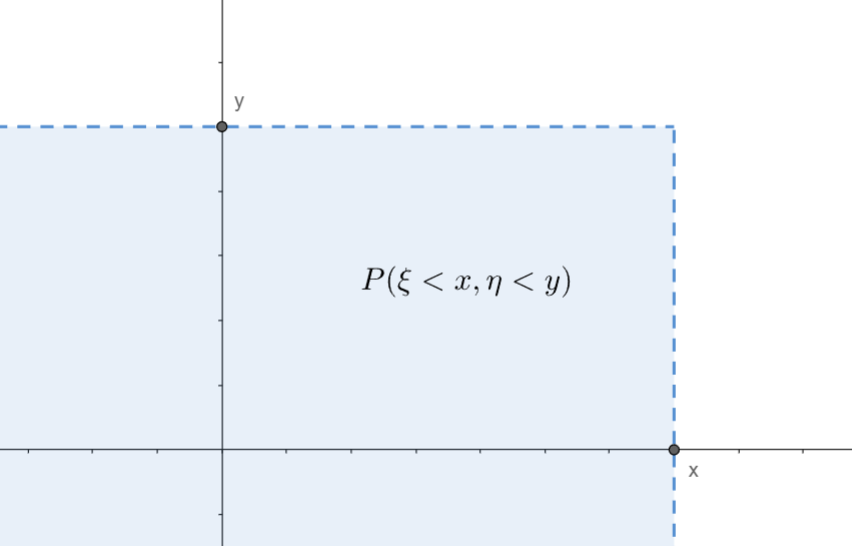
\includegraphics[width=0.55\textwidth]{probtheory/images/probtheory_2024_11_19_1}
    \end{center}


    \subsubsection{Свойства функции распределения}

    \begin{enumerate}
        \item $0 \leq F_{\xi, \eta}(x, y) \leq 1$
        \item $F_{\xi, \eta}(x, y)$ - неубывающая по каждому аргументу
        \item $\lim_{x \to -\infty} F_{\xi, \eta}(x, y) = \lim_{y \to -\infty} F_{\xi, \eta}(x, y) = 0, $
        $\lim_{\substack{x \to \infty \\ y \to \infty}} F_{\xi, \eta}(x, y) = 1$

        \item Восстановление маргинального (частного) распределения: 
        $\lim_{x \to \infty} F_{\xi, \eta}(x, y) = F_\eta(y)$, и наоборот - $\lim_{y \to \infty} F_{\xi, \eta}(x, y) = F_\xi(x)$

        \item $F_{\xi, \eta}(x, y)$ - непрерывна слева по каждому аргументу

        \item $P(x_1 \leq \xi < x_2, y_1 \leq \eta < y_2) = F_{\xi, \eta}(x_2, y_2) - F_{\xi, \eta}(x_2, y_1) - F_{\xi, \eta}(x_1, y_2) + F_{\xi, \eta}(x_1, y_1)$
    \end{enumerate}

    \subsection{Независимость случайных величин}

    \Def Случайные величины $\xi_1, \dots, \xi_n$ независимы в совокупности, если для любого набора Борелевских множеств из
    $\mathcal{B}(\Real^n)$, $B_1, B_2, \dots, B_n$

    $p(\xi_1 \in B_1, \xi_2 \in B_2, \dots, \xi_n \in B_n) = p(\xi_1 \in B_1) \cdot p(\xi_2 \in B_2) \cdot \dots \cdot p(\xi_n \in B_n)$

    \Def Случайные величины $\xi_1, \xi_2, \dots, \xi_n$ попарно независимы, если независимы любые две из них

    \Notas Из независимости в совокупности следует попарная независимость: 

    $\xi_1, \dots, \xi_n$ независимы в совокупности, тогда покажем $\forall i, j \ \xi_i$ и $\xi_j$ - независимы

    Возьмем набор $B_i, B_j \in \mathcal{B}(\Real^n)$, при $k \neq i, j \ B_k = \Real$ \hfill $P(\xi_k \in B_k) = 1$

    Тогда $p(\xi_1 \in B_1, \dots, \xi_n \in B_n) = P(\xi_i \in B_i, \xi_j \in B_j) = P(\xi_i \in B_i) \cdot P(\xi_j \in B_j)$

    \Nota Из попарной независимости не следует независимость в совокупности, как видно из примера Берншейна

    Под независимыми величинами будем понимать независимые в совокупности

    \subsection{Дискретная система двух случайных величин}

    \Def Случайные величины $\xi, \eta$ имеют совместное дискретное распределение, если случайный вектор $(\xi, \eta)$
    принимает не более, чем счетное число значений, то есть существует конечный или счетный набор пар чисел $(x_i, y_i)$, 
    таких что $P(\xi = x_i, \eta = y_i) > 0, \sum_{i, j} P(\xi = x_i, \eta = y_i) = 1$

    Таким образом двумерная дискретная случайная величина задается законом распределения - таблице вероятностей

    \begin{tabular}{c|c|c|c|c}
        $\xi \backslash \eta$ & $y_1$ & $y_2$ & $\dots$ & $y_m$ \\
        \hline
        $x_1$ & $p_{11}$ & $p_{12}$ & $\dots$ & $p_{1m}$ \\
        \hline
        $x_2$ & $p_{21}$ & $p_{22}$ & $\dots$ & $p_{2m}$ \\
        \hline
        $\vdots$ & $\vdots$ & $\vdots$ & $\ddots$ & $\vdots$ \\
        \hline
        $x_n$ & $p_{n1}$ & $p_{n2}$ & $\dots$ & $p_{nm}$ \\
    \end{tabular}

    Условие нормировки: $\sum_{i, j} p_{i, j} = 1$

    Зная общий закон распределения, можно восстановить частное (маргинальное) распределение по формулам: 

    $p_i = \sum_{j = 1}^m p_{i, j} \qquad q_j = \sum_{i = 1}^n p_{i, j}$

    \Def Дискретные случайные величины $\xi_1, \xi_2, \dots, \xi_n$ независимы, если для любых $x_1, x_2, \dots, x_n$ 
    $p(\xi_1 = x_1, \xi_2 = x_2, \dots, \xi_n = x_n) = p(\xi_1 = x_1) \cdot p(\xi_2 = x_2) \cdot \dots \cdot p(\xi_n = x_n)$

    При $n = 2$: $p_{i, j} = p_i \cdot q_j \ \forall i, j$

    \Ex

    \begin{tabular}{c|c|c|c|c}
        $\xi \backslash \eta$ & $-1$ & $0$ & $1$ & $p_i$ \\
        \hline
        $-1$ & $0.1$ & $0.2$ & $0.1$ & $0.4$ \\
        \hline
        $2$ & $0.2$ & $0.3$ & $0.1$ & $0.6$ \\
        \hline
        $q_j$ & $0.3$ & $0.5$ & $0.2$ & $\Sigma = 1$ \\
    \end{tabular}

    Найти маргинальное распределение и проверить независимость случайных величин


    \begin{tabular}{c|c|c}
        $\xi$ & $-1$ & $2$ \\
        \hline
        $p_i$ & $0.4$ & $0.6$  \\
    \end{tabular}

    \begin{tabular}{c|c|c|c}
        $\eta$ & $-1$ & $0$ & $1$ \\
        \hline
        $q_j$ & $0.3$ & $0.5$ & $0.2$  \\
    \end{tabular}

    $p_{11} = 0.1 \neq 0.12 = p_1 \cdot q_1 \qquad \Longrightarrow \xi, \eta$ - зависимы

    \subsection{Абсолютно непрерывная система двух случайных величин}

    \Def Случайные величины $\xi$ и $\eta$ имеют абсолютно непрерывное совместное распределение, если
    $\exists f_{\xi, \eta}(x, y)$, такая что $\forall B \in \mathcal{B}(\Real^2) \ P((\xi, \eta) \in B) = \iint_B f_{\xi, \eta}(x, y) dxdy$

    Функцию $f_{\xi, \eta}(x, y)$ будем называть функцией плотности совместного распределения случайных величин $\xi$ и $\eta$

    \underline{Геометрический смысл} плотности: 

    % картиночка

    \underline{Свойства} плотности:

    \begin{enumerate}
        \item $f_{\xi, \eta}(x, y) \leq 0$
        \item Условие нормировки: $\iint_{\Real^2} f_{\xi, \eta}(x, y) dxdy = 1$
        \item $F_{\xi, \eta} = \int_{-\infty}^x \int_{-\infty}^y f_{\xi, \eta}(x, y) dydx$

        \item $f_{\xi, \eta}(x, y) = \frac{\partial^2 F_{\xi, \eta}(x, y)}{\partial x \partial y}$
        
        \item Если случайные величины $\xi, \eta$ имеют абсолютно непрерывное совместное распределение с плотностью $f(x, y)$, 
        то маргинальное распределение величин $\xi, \eta$ также имеют абсолютно непрерывное распределение
        с плотностями $f_\xi(x) = \int_{-\infty}^\infty f_{\xi, \eta}(x, y) dy, f_\eta(y) = \int_{-\infty}^\infty f_{\xi, \eta}(x, y) dx$

        \begin{MyProof}
            $F_{\xi}(x) = \lim_{y \to \infty} F_{\xi, \eta}(x, y) = \int_{-\infty}^x \int_{-\infty}^\infty f(x, y) dydx$

            Из этого $\int_{-\infty}^\infty f(x, y) = f_\xi(x)$
        \end{MyProof}

        \item Так как вероятность попадания в Борелевские множества полностью задается функцией распределения, 
        то условие независимости случайных величин эквивалентно следующему:

        $\xi_1, \xi_2, \dots, \xi_n$ независимы, если функция общего распределения распадается в произведение 
        отдельных функцию распределения
    
        $F_{\xi_1, \xi_2, \dots, \xi_n}(x_1, x_2, \dots, x_n) = F_{\xi_1}(x_1) \cdot F_{\xi_2}(x_2) \cdot \dots \cdot F_{\xi_n}(x_n)$

        \item \textit{Равносильное определение}: абсолютно непрерывные случайные величины $\xi_1, \dots, \xi_n$ независимы в совокупности тогда и только тогда, 
        когда плотность совместного распределения $f_{\xi_1, \xi_2, \dots, \xi_n}(x_1, x_2, \dots, x_n) = f_{\xi_1}(x_1) \cdot f_{\xi_2}(x_2) \cdot \dots \cdot f_{\xi_n}(x_n)$
    
        \begin{MyProof}
            При $n = 2$ случайные величины $\xi$ и $\eta$ независимы $\Longleftrightarrow F_{\xi, \eta}(x, y) = F_\xi(x) \cdot F_\eta(y) = \int_{-\infty}^x f_\xi(x) dx \cdot \int_{-\infty}^y f_\eta(y) dy = \int_{-\infty}^x \int_{-\infty}^y f_\xi(x) \cdot f_\eta(y) dxdy \Longrightarrow f_{\xi,\eta}(x, y) = f_\xi(x)f_\eta(y)$

            Аналогично для высших размерностей
        \end{MyProof}

    \end{enumerate}

    \Nota Совместное распределение абсолютно непрерывных случайных величин не обязано быть абсолютно непрерывным, оно может быть сингулярным

    \Exs Бросаем точку на отрезок прямой $y = x$ ($0 \leq x, y \leq 1$), $\xi$ - абсцисса точки, $\eta$ - ордината точки

    Случайный вектор $(\xi, \eta)$ имеют сингулярное распределение (непрерывное с нулевой областью) - 
    так как число элементарных исходов несчетно, но мера Лебега в $\Real^2$ отрезка равна 0

    \Nota Совместное распределение $\xi_1, \xi_2, \dots, \xi_n$ будет сингулярным, если одна из координат является функцией других (наблюдается функциональная зависимость)

    \subsection{Многомерное равномерное распределение}

    \Def $\letsymbol D \subset \Real^n$ - Борелевское множество в $\Real^n$ с конечной мерой Лебега ($0 < \lambda(D) < \infty$),
    случайный вектор $(\xi_1, \dots, \xi_n)$ имеет равномерное распределение, если плотность совместного распределения 
    постоянна в данной области и равна нулю вне данной области

    $f_{\xi_1, \dots, \xi_n}(x_1, \dots, \x_n) = \begin{cases}\frac{1}{\lambda(D)}, & \text{если } (x_1, \dots, x_n) \in D \\ 0, & \text{если } (x_1, \dots, x_n) \not\in D\end{cases}$
% end probtheory_2024_11_19.tex

% begin probtheory_2024_11_26.tex

    \section{Лекция 13}

    \subsection{Математическое ожидание и дисперсия случайного вектора}
    
    $\letsymbol \vec{\xi} = (\xi_1, \dots, \xi_n)$ - случайный вектор, 
    $\forall 1 \leq i \leq n \ \xi_i$ - случайная величина

    \Def Математическим ожиданием случайного вектора называется вектор с координатами 
    из математических ожиданий его компонент: $E\vec{\xi} = (E\xi_1, \dots, E\xi_n)$

    \Def Дисперсией (или матрицей ковариаций) случайного вектора называется матрица
    $D\vec{\xi} = E(\vec{\xi} - E\vec{\xi})^T \cdot (\vec{\xi} - E\vec{\xi})$, состоящая
    из элементов $d_{i, j} = \cov (\xi_i, \xi_j)$. В частности $d_{i, i} = \cov (\xi_i, \xi_i) = D\xi_i$

    \subsection{Функции от двух случайных величин}

    \begin{MyTheorem}
        \Ths Пусть $\xi_1, \xi_2$ - случайные величины с общем плотностью $f_{\xi_1, \xi_2}(x, y)$, и есть функция
        $g(x, y) \ : \ \Real^2 \rightarrow \Real$. Тогда случайная величина $\eta = g(\xi_1, \xi_2)$ имеет
        функцию распределения $F_{\eta}(z) = \iint_{D_z} f(x, y)dxdy$, 
        где $D_z = \{(x, y) \in \Real^2 \ | \ g(x, y) < z\}$
    \end{MyTheorem}

    \begin{MyProof}
        $F_\eta = p(\eta < z) = p(g(\xi_1, \xi_2) < z) = p((\xi_1, \xi_2) \in D_z) = \iint_{D_z} f(x, y) dxdy$
    \end{MyProof}

    \begin{minipage}{\textwidth}
        \begin{wrapfigure}{r}{0pt}
            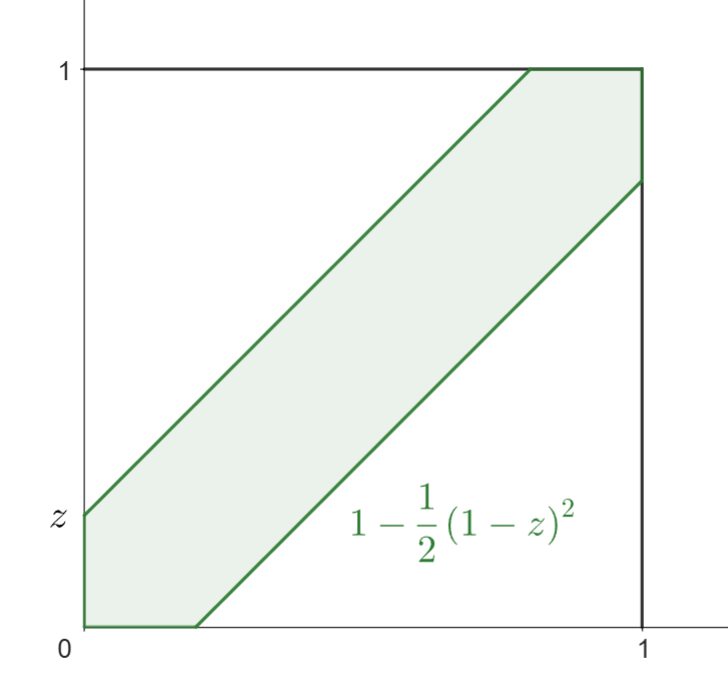
\includegraphics[width=5cm]{probtheory/images/probtheory_2024_11_26_1}
        \end{wrapfigure}

        \ExN{Задача о встрече} двое договорились встретится между 12:00 и 13:00. Случайная величина $\eta$ - 
        время ожидания. Найти функцию распределения

        $\xi_1$ - время прихода первого, $\xi_2$ - второго; $\xi_1, \xi_2 \in U(0, 1)$, они независимы, 
        $\forall x, y \in [0, 1] \ f_{\xi_1}(x) = 1, f_{\xi_2}(y) = 1$

        Поэтому $f_{\xi_1, \xi_2}(x, y) = f_{\xi_1}(x) f_{\xi_2}(y) = 1, (x, y) \in [0, 1] \times [0, 1]$

        $\eta = |\xi_1 - \xi_2| \Longrightarrow D_z = \{(x, y) \in \Real^2 \ | \ |x - y| < z\}$

        $F_\eta = \iint_{D_z} f_{\xi_1, \xi_2}(x, y) dxdy = \iint_{D_z} dxdy = 1 - 2 \cdot \frac{1}{2} (1 - z)^2 = 
        2z - z^2, \ z \in [0, 1]$
    \end{minipage}

    \begin{MyTheorem}
        \Ths $\letsymbol \xi_1, \xi_2$ - независимые абсолютно непрерывные случайные величины с плотностями
        $f_{\xi_1}(x)$ и $f_{\xi_2}(y)$

        Тогда плотность суммы $\xi_1 + \xi_2$ равна $f_{\xi_1 + \xi_2}(t) \int_{-\infty}^\infty 
        \underset{\text{т. н. свертка}}{\underbrace{f_{\xi_1}(x) f_{\xi_2}(t - x)}} dx$
    \end{MyTheorem}

    \begin{MyProof}
        \begin{minipage}{\textwidth}
            \begin{wrapfigure}{r}{0pt}
                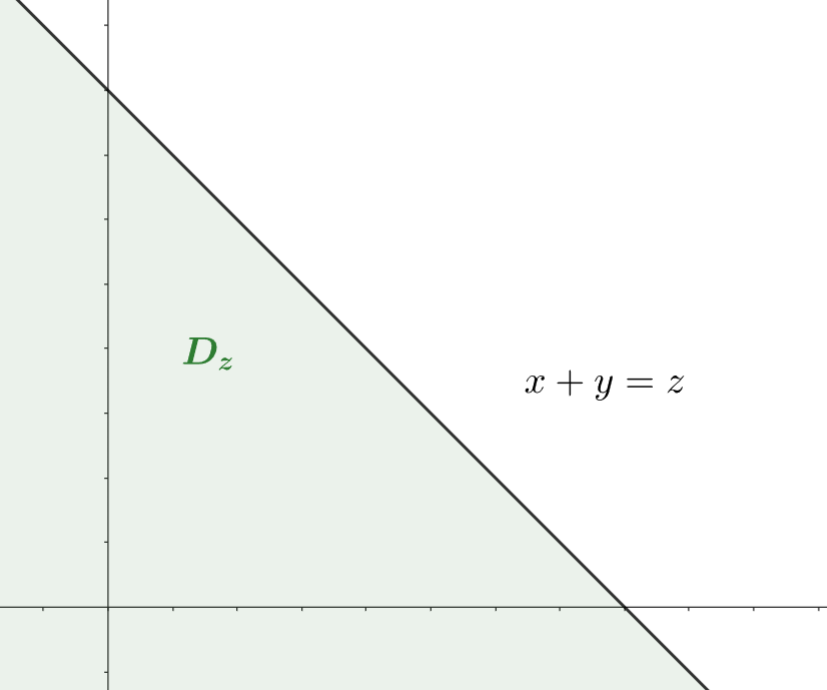
\includegraphics[width=5cm]{probtheory/images/probtheory_2024_11_26_2}
            \end{wrapfigure}
            
            Так как случайные величины $\xi_1$ и $\xi_2$ независимы, то $f_{\xi_1, \xi_2}(x, y) = f_{\xi_1}(x) f_{\xi_2}(y)$

            И согласно предыдущей теореме $F_{\xi_1 + \xi_2}(z) = \iint_{D_z} f_{\xi_1, \xi_2}(x, y) dxdy = 
            \iint_{D_z} f_{\xi_1}(x)f_{\xi_2}(y) dxdy$, где $D_z = \{(x, y) \in \Real^2 \ | \ x + y < z\}$

            $F_{\xi_1 + \xi_2}(z) = \int_{-\infty}^\infty dx \int_{-\infty}^{z - x} f_{\xi_1}(x)f_{\xi_2}(y) dy = \\
            \left[\begin{matrix}y = t - x; & dy = dt; & t = y + x \\ t(-\infty) = -\infty; & t(z - x) = z & \end{matrix}\right] = \\
            \int_{-\infty}^{\infty} f_{\xi_1}(x) dx \int_{-\infty}^z f_{\xi_2}(t - x) dt = \\
            \int_{-\infty}^z \left(\int_{-\infty}^\infty f_{\xi_1}(x)f_{\xi_2}(t - x) dx\right) dt \Longrightarrow
            f_{\xi_1 + \xi_2}(t) = \int_{-\infty}^\infty f_{\xi_1}(x)f_{\xi_2}(t - x) dx$
        \end{minipage}
    \end{MyProof}

    Следствие: сумма двух независимых абсолютно непрерывных случайных величин также имеет абсолютно 
    непрерывное распределение

    \Notas Условие независимости существенно, контр-пример: $\xi_1; \xi_2 = -\xi_1$, тогда $\xi_1 + \xi_2 \equiv 0$

    \subsection{Сумма стандартных распределений. Устойчивость относительно суммирования}

    \Def Если сумма двух независимых случайных величин одного типа распределения также будет этого же типа,
    то говорят, что распределение устойчиво относительно суммирования

    \ExN{1} $\xi \in B_{n, p}; \eta \in B_{m, p}$. Тогда ясно, что $\xi + \eta \in B_{n + m, p}$ 
    (по определению биномиального распределения $B_{n, p}$ - число успехов из $n$ испытаний, где $p$ - вероятность успеха)

    \ExN{2} $\xi \in \Pi_{\lambda}, \eta \in \Pi_{\mu}$, они независимы. Тогда $\xi + \eta \in \Pi_{\lambda + \mu}$

    \begin{MyProof}
        $\xi + \eta = 0, 1, 2, 3, \dots \quad \letsymbol k \geq 0$. 
        Тогда $p(\xi + \eta = k) = \sum^k_{i = 0} P(\xi = i, \eta = k - i) = 
        \sum^k_{i = 0} P(\xi = i) P(\eta = k - i) = \sum_{i = 0}^k \frac{\lambda^i}{i!} e^{-\lambda} \frac{\mu^{k - i}}{(k - i)!} e^{-\mu} = 
        e^{-\lambda - \mu} \sum_{i = 0}^k \frac{\lambda^i \mu^{k - i}}{i! (k - i)!} = 
        e^{-\lambda - \mu} \frac{1}{k!} \sum_{i = 0}^k \frac{\lambda^i \mu^{k - i} k!}{i! (k - i)!} = 
        e^{-\lambda - \mu} \frac{1}{k!} \sum_{i = 0}^k \lambda^i \mu^{k - i}C_k^i = 
        e^{-\lambda - \mu} \frac{(\lambda + \mu)^k}{k!} \Longrightarrow \xi + \eta \in \Pi_{\lambda + \mu}$
    \end{MyProof}

    \ExN{3} $\xi, \eta \in N(0, 1)$ и независимы. Тогда $\xi + \eta \in N(0, 2)$

    \begin{MyProof}
        $f_{\xi}(x) = \frac{1}{\sqrt{2\pi}} e^{-\frac{x^2}{2}}; f_\eta(y) = \frac{1}{\sqrt{2\pi}} e^{-\frac{y^2}{2}}$

        По формуле свертки $f_{\xi + \eta}(t) = \int_{-\infty}^{\infty} \frac{1}{\sqrt{2\pi}} e^{-\frac{x^2}{2}} \frac{1}{\sqrt{2\pi}} e^{-\frac{(t - x)^2}{2}} = 
        \frac{1}{2\pi} \int e^{-(x^2 - tx + \frac{t^2}{2})} = \frac{1}{2\pi} e^{-\frac{t^2}{4}} \int_{-\infty}^\infty e^{-(x^2 - tx + \frac{t^2}{4})} dx = 
        \frac{1}{2\pi} e^{-\frac{t^2}{4}} \int_{-\infty}^\infty e^{-(x - \frac{t}{2})^2} d(x - \frac{t}{2}) = 
        \frac{1}{2\pi} e^{-\frac{t^2}{4}} \sqrt{\pi} = \frac{1}{\sqrt{2}\sqrt{2\pi}} e^{-\frac{t^2}{2(\sqrt{2})^2}} 
        \Longrightarrow \xi + \eta \in N(0, 2)$
    \end{MyProof}

    \ExN{4} В общности для независимых $\xi \in N(a_1, \sigma^2_1), \eta \in N(a_2, \sigma_2^2) \ \xi + \eta \in N(a_1 + a_2, \sigma_1^2 + \sigma_2^2)$ 

    \ExN{5} Равномерное распределение неустойчиво относительно суммирования, контрпример:

    $\xi, \eta \in U(0, 1)$ - независимы

    $\forall x, y \in [0, 1] \ f_{\xi}(x) = 1, f_\eta(y) = 1$ и $f_{\xi, \eta}(x, y) = 1$

    По первой теореме $F_{\xi, \eta}(x, y) = \iint_{D_z} f_{\xi, \eta}(x, y) dxdy = \iint_{D_z} dxdy = S_{D_z}$, где $D_z = \{(x, y) \ | \ x + y < z\}$

    \mediumvspace

    \begin{multicols}{2}
        \begin{center}
            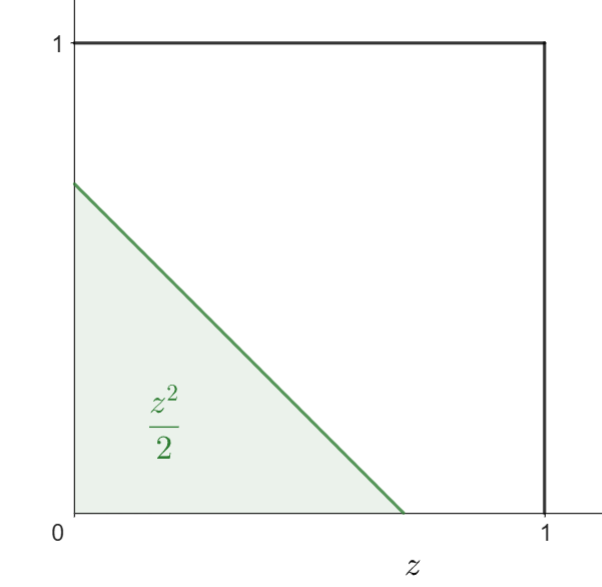
\includegraphics[height=6cm]{probtheory/images/probtheory_2024_11_26_3}

            а) $0 < z \leq 1$
        \end{center}

        \begin{center}
            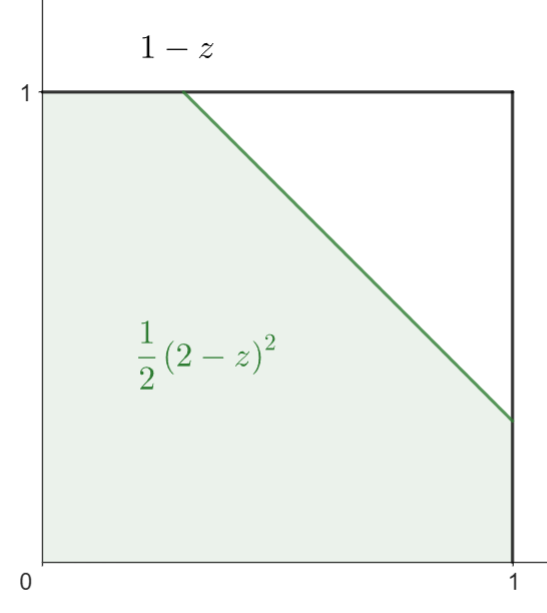
\includegraphics[height=6cm]{probtheory/images/probtheory_2024_11_26_4}

            б) $1 < z \leq 2$
        \end{center}
    \end{multicols}

    \smallvspace

    $S_{D_z} = \begin{cases}0, & z < 0 \\ \frac{z^2}{2}, & 0 \leq z \leq 2 \\ 1 - \frac{1}{2}(2 - z)^2 & 1 \leq z \leq 2 \\ 0, & z > 2\end{cases}$

    $f_{\xi + \eta}(z) = \begin{cases}0, & z < 0 \\ z, & 0 \leq z \leq 2 \\ 2 - z & 1 \leq z \leq 2 \\ 0, & z > 2\end{cases} \not\equiv C \Longrightarrow \xi + \eta$ не имеют равномерное распределение

    \Nota FUN FACT: сумма нескольких величин с равномерным распределением приближается к нормальному распределению

    \subsection{Условное распределение}

    \Def Условным распределением случайной величины из системы случайных величин $(\xi, \eta)$ 
    называется ее распределение, найденное при условии, что другая случайная величина приняла 
    определенное значение. Обозначается $\xi | \eta = y$

    \DefN{A}: Условным математическим ожиданием (обозначается $E(\xi | \eta = y)$) называется 
    математическим ожиданием случайной величины $\xi$ при соответствующем условном распределении

    \subsubsection{I. Условное распределение в дискретной системе двух случайных величин}

    Пусть $(\xi, \eta)$ задана законом распределения:

    \begin{tabular}{c|c|c|c|c}
        $\xi \backslash \eta$ & $y_1$ & $y_2$ & $\dots$ & $y_m$ \\
        \hline
        $x_1$ & $p_{11}$ & $p_{12}$ & $\dots$ & $p_{1m}$ \\
        \hline
        $x_2$ & $p_{21}$ & $p_{22}$ & $\dots$ & $p_{2m}$ \\
        \hline
        $\vdots$ & $\vdots$ & $\vdots$ & $\ddots$ & $\vdots$ \\
        \hline
        $x_n$ & $p_{n1}$ & $p_{n2}$ & $\dots$ & $p_{nm}$ \\
    \end{tabular}

    Формула условной вероятности: $P(A | B) = \frac{P(AB)}{P(B)}$

    Вероятности условных распределений считаем по формулам:

    $\xi | \eta = y_j$: $p_i = p(\xi = x_i \ | \ \eta = y_j) = \frac{p(\xi = x_i, \eta = y_j)}{p(\eta = y_j)} = \frac{p_{ij}}{q_j}$

    $\eta | \xi = x_i$: $q_j = p(\eta = y_j \ | \ \xi = x_i) = \frac{p(\xi = x_i, \eta = y_j)}{p(\xi = x_i)} = \frac{p_{ij}}{p_i}$

    То есть вероятность в соответствующем столбце делим на 

    \subsubsection{II. Условное распределение в непрерывной системе двух случайных величин}

    Пусть $(\xi, \eta)$ задана плотностью $f_{\xi, \eta}(x, y)$ совместного распределения, тогда плотность 
    условного распределения $\xi | \eta = y$: 

    $f(x | y) = \frac{f_{\xi, \eta}(x, y)}{\int_\Real f_{\xi, \eta}(x, y)dx} = \frac{f_{\xi, \eta}(x, y)}{f_{\eta}(y)}$

    \Def Функция $f(x | y) = \frac{f_{\xi, \eta}(x, y)}{f_{\eta}(y)}$ называется условной плотностью

    \Def Условное математические ожидание вычисляется по формуле $E(\xi | \eta = y) = \int_{-\infty}^\infty xf(x | y)dx$

    Аналогично $E(\eta | \xi = x) = \int_{-\infty}^\infty yf(y | x)dy$

    \Nota При фиксированном значении $x$ $f(y | x)$ зависит только от $y$, а $E(\eta | \xi = x) \in \Real$. 
    Если рассматривать $x$ как переменную, то условное математическое ожидание $E(\eta | \xi = x)$ является
    функцией от $x$ и называется функцией регрессии $\eta$ на $\xi$. График такой функции называют линией регрессии

    \Nota Так как значение $x$ - значение случайной величины $\xi$, то условное матожидание $E(\eta | \xi = x)$ 
    можно рассматривать как случайную величину
% end probtheory_2024_11_26.tex



\end{document}

